\subsection{Messungen}
In diesem Abschnitt sollen charakteristische Messwerte der Fahrspurerkennung, Regelung, sowie dem Zusammenspiel beider Komponenten dargestellt und diskutiert werden. Dies soll unter Veränderung der Umgebungsbedingungen sowie mit unterschiedlichen Fortbewegungsgeschwindigkeiten des Modellfahrzeugs geschehen.
  
\subsubsection{Evaluation ohne Ground Truth}
Für die Detektion von Fahrspuren auf Einzelbildern und die daraus resultierende Bewegung des Fahrzeugs existieren zum jetzigen Zeitpunkt keine Vergleichswerte. 

\paragraph{Bildverarbeitung} 
Für ein Benchmark der Fahrspurerkennung könnte ein Ground-Truth-Datensatz in Form von Bildern mit richtig eingetragen Fahrbahnmarkierungen die präziseste Bewertung hervorbringen. Da die Erstellung eines solchen jedoch sehr zeitaufwendig ist, wurde eine leichter automatisierbare Methode der Evaluation gewählt.

Durch die implementierte Verifikation der erkannten Koordinatenserien kann eine Fehlerkennung weitgehend ausgeschlossen werden. Den deutlichsten Indikator für ein falsch verarbeitetes Bild stellt also eine nicht oder nur auf einem sehr kurzen Abschnitt detektierte Fahrbahnmarkierung dar. Den Grenzwert der Länge für eine fehlerhaft erkannte Linie ist oft unkritisch, da der Detektionsalgorithmus in den meisten Fällen zufriedenstellend funktioniert oder schon bei kurzer Linienlänge fehlschlägt. Wir haben uns dafür entschieden etwa die halbe Sichtweite des Fahrzeugs (ab Stoßstange bis Bildrand) als Schwellwert anzusehen.

\paragraph{Regelung} 
Die Güte der Regelung bzw. des Zusammenspiels aus Bildverarbeitung und Regelung könnte am exaktesten durch ein hinreichend genaues System zur Lokalisierung des Fahrzeugs im Testszenario ermittelt werden. Somit wäre es möglich die Abweichung der gefahrenen Strecke von einer vorgegebenen Ideallinie auszuwerten. Da die Inbetriebnahme des an der Professur vorhandenen zweidimensionalen Tracking-Systems viel Einarbeitungszeit benötigt, wird hier auf eine einfache Methode zurückgegriffen. Es wird lediglich vermerkt ob das Fahrzeug die Fahrspur völlig verlässt oder dem Straßenverlauf zufriedenstellend folgt.

\subsubsection{Überlegungen zur Darstellung der Messwerte}
Um möglichst viele Informationen kompakt abzubilden wurden unter anderem die Diagrammtypen Boxplot sowie Histogramm genutzt. Da kurz nach dem Start des Fahrzeugs 
\begin{itemize}
\item
MATLAB viele Funktionen erst noch in den Hauptspeicher laden muss (\glqq Warmlaufphase\grqq\ )
\item
Das Fahrzeug vor vollendeter Verarbeitung des ersten Bildes schon ohne gültigen Zielpunkt losfährt
\end{itemize}
wurden diese nicht-repräsentativen Phasen in den entsprechenden Grafiken ausgelassen, da sie die Aussagekraft der Messwerte beeinträchtigen würden.

\subsubsection{Parametertuning}
Dieser Paragraph beschäftigt sich mit der Ermittlung der maximal fahrbaren Geschwindigkeit bei Nutzung der entwickelten Bildverarbeitungs- und Regelungsstruktur. Durch die Auswertung verschiedener Messwerte soll der \glqq Flaschenhals\grqq\ gefunden und, wenn möglich, durch Parameteranpassung beseitigt werden.

Wichtige, noch anzupassende Parameter stellen dar:
\begin{itemize}
\item Die Frequenz, in der Bilder verarbeitet werden
\item Die Frequenz, mit der die Regelung stattfindet
\item Die Entfernung des Zielpunktes der Regelung vom Fahrzeug
\end{itemize}

Den Ausganspunkt für die folgenden Optimierungen bildet eine Geschwindigkeit von
\SI{0.1}{\metre\per\second}. Die Frequenz, mit welcher die Bilder verarbeitet werden wurde auf \SI{1}{\hertz} festgelegt, da die Extraktion der Linienpunkte eines Testbildes ca. \SI{0.5}{\second} benötigt. Die Frequenz der Regelung wurde initial auf \SI{20}{\hertz} festgelegt, da der Rechenaufwand für einen Regelungszyklus sehr gering ist. Eine noch höhere Regelfrequenz verspricht keinen Performancegewinn und läge schon nahe der maximalen Ansteuerfrequenz des Lenkservos sowie der Abtastrate der \gls{acr:imu} (jeweils \SI{50}{\hertz}).

Mithilfe dieser Einstellung absolvierte das Fahrzeug erfolgreich eine Runde im Testparcours. Wie in Abb.~\ref{fig:evaluation:riverflow:times_combined_1Hz_0_1m_s_over_piciter} zu sehen, benötigt ein Bild-Callback im Echtzeitbetrieb, d.h. bei mehrmaliger Ausführung erheblich weniger Zeit als beim einmaligen Messung anhand eines Testbildes. Die Verringerung der Bearbeitungsdauer \scl{t_{img}} von ca. \SI{500}{\milli\second} auf \SI{128}{\milli\second} (Median der in Abb.~\ref{fig:evaluation:riverflow:times_combined_1Hz_0_1m_s_over_piciter} dargestellten Daten) lässt sich unter anderem durch die Fahigkeit MATLABs, Funktionen bei wiederholter Ausführung im Hauptspeicher zu halten und somit schneller ausführen zu können, erklären. Eine signifikante Erhöhung der Bildfrequenz \scl{f_{img}} ist also möglich. Nimmt man die vom der Regelung und Posenaktualisierung, d.h. dem Odometrie-Callback  pro Sekunde benötigte Zeit \scl{t_{odom-per-sec}} als konstant an, lässt sich die theoretisch mögliche Bildfrequenz wie folgt berechnen:
\begin{subequations}
\begin{equation}
	T_{img} = t_{img}+t_{odom-per-sec}\cdot T_{img}
\end{equation}
%\begin{equation}
%	T_{img}\cdot(1-t_{odom-per-sec}) = t_{img}
%\end{equation}
\begin{equation}
	T_{img} = \frac{t_{img}}{1-t_{odom-per-sec}}
\end{equation}
\begin{equation}	
	f_{img} = \frac{1}{T_{img}}
\end{equation}
\end{subequations} 
Mit einer Bildbearbeitungszeit \(t_{img}=\SI{128}{\milli\second}\) sowie dem Zeitbedarf des Odometrie-Callbacks von \(t_{odom-per-sec}=\SI{262}{\milli\second\per\second}\) ergibt sich eine in der Theorie nutzbare Framerate von über \SI{5}{\hertz}. Mit dieser Bildfrequenz wurde eine weitere Testfahrt absolviert, in Abb. \ref{fig:evaluation:riverflow:times_pic_5Hz_0_2m_s_over_piciter} wird die bessere Nutzung der zur Verfügung stehenden Rechenzeit deutlich. Abbildung \ref{fig:evaluation:riverflow:times_pic_5Hz_0_2m_s_over_piciter} zeigt jedoch, dass die Periodendauer der Bildverarbeitung zwischen 2 Punkten oszilliert. Der erwartete zeitliche Abstand zweier konsekutiver Aufnahmen von \SI{200}{ms} wird häufig nicht erreicht, stattdessen befindet sich ein Abstand von \(2 \cdot \SI{200}{ms} = \SI{400}{ms}\) zwischen aufeinander folgenden Bildern. Dies führt zu dem Schluss, dass durch nicht vorhandene Pufferung Aufnahmen ausgelassen wurden.

\begin{figure}[ht] % [htb]
\centering
\subfloat[\SI{5}{\hertz}\label{fig:evaluation:riverflow:times_pic_5Hz_0_2m_s_over_piciter}]{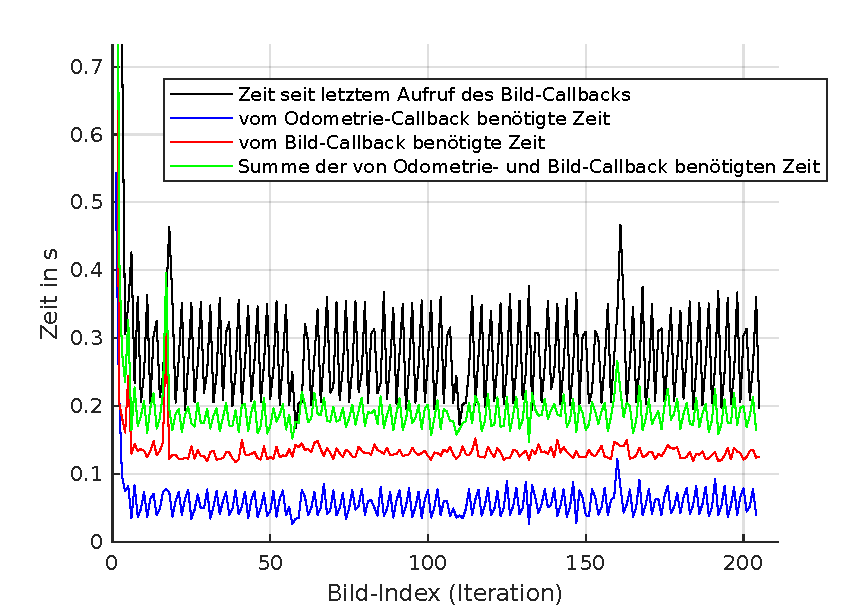
\includegraphics[width=0.45\textwidth]{evaluation_riverflow_times_combined_5Hz_0_2m_s_over_piciter}}
\qquad
\subfloat[\SI{4}{\hertz}\label{fig:evaluation:riverflow:times_pic_4Hz_0_2m_s_over_piciter}]{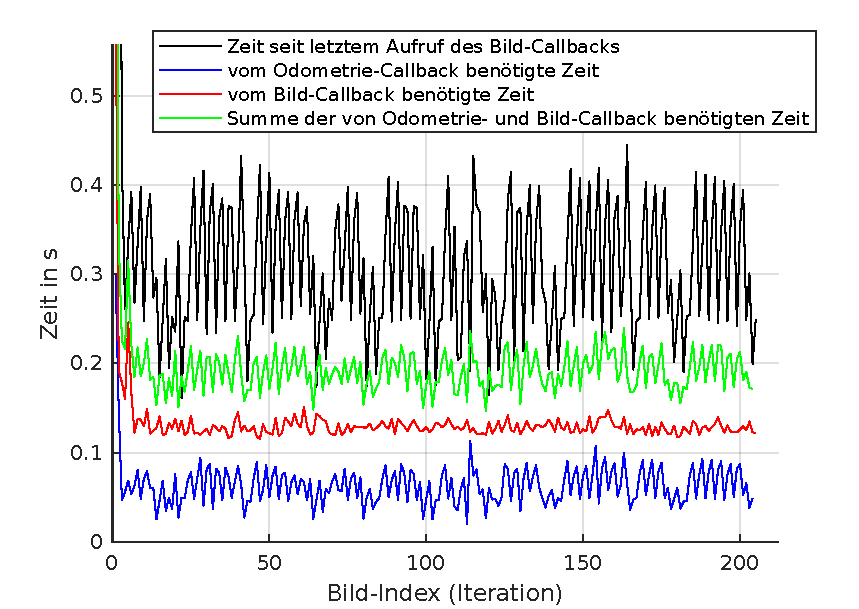
\includegraphics[width=0.45\textwidth]{evaluation_riverflow_times_combined_4Hz_0_2m_s_over_piciter}}
\qquad
\subfloat[\SI{3}{\hertz}\label{fig:evaluation:riverflow:times_pic_3Hz_0_2m_s_over_piciter}]{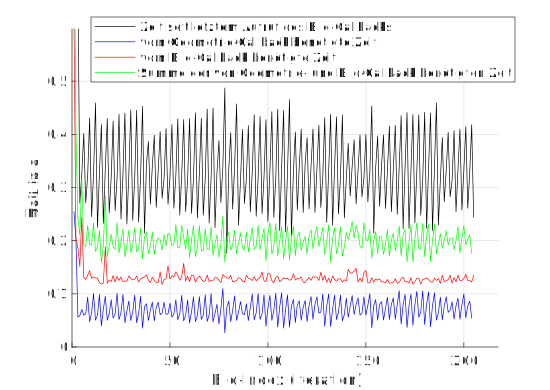
\includegraphics[width=0.45\textwidth]{evaluation_riverflow_times_combined_3Hz_0_2m_s_over_piciter}}
\subfloat[\SI{1}{\hertz}\label{fig:evaluation:riverflow:times_combined_1Hz_0_1m_s_over_piciter}]{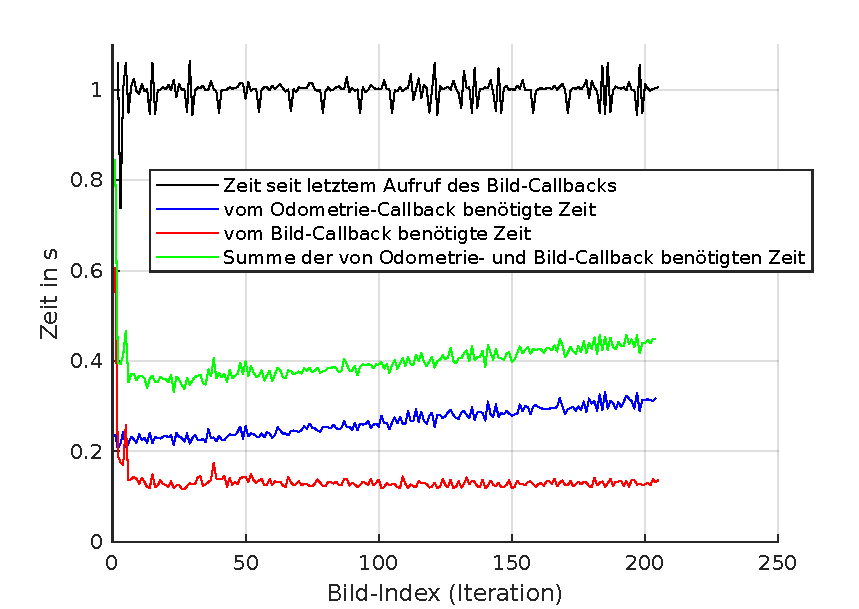
\includegraphics[width=0.45\textwidth]{evaluation_riverflow_times_combined_1Hz_0_1m_s_over_piciter}}
\caption{Zeitbedarf aller Fahrspurverfolgungskomponenten bei \SIlist{5;4;3;1}{\hertz} Bildfrequenz}
\end{figure}

Im folgenden wurde die Bildfrequenz zuerst auf 4 (s.Abb. \ref{fig:evaluation:riverflow:times_pic_4Hz_0_2m_s_over_piciter}), später auf \SI{3}{\hertz} verringert (s.Abb. \ref{fig:evaluation:riverflow:times_pic_3Hz_0_2m_s_over_piciter}). Erst jetzt konnte kein Springen der Periodendauer des Bild-Callbacks auf ein Vielfaches seines Erwartungswertes mehr festgestellt werden. Eine leichte Oszillation des zeitlichen Abstands zweier Aufnahmen ist auch in Abb. \ref{fig:evaluation:riverflow:times_pic_3Hz_0_2m_s_over_piciter} zu erkennen, jedoch beträgt der Mittelwert fast exakt die erwarteten \SI{333}{ms}. Die verbleibenden Unregelmäßigkeiten sind auf den Kamera-Node, welcher die Bilder aufnimmt und im entsprechenden Topic veröffentlicht, hervorgerufen werden (s. Abschnitt \ref{ssec:software_struktur:ros:nodes}). Abbildung \ref{fig:evaluation:riverflow:times_combined_3Hz_0_2m_s_pie_median} bzw. \ref{fig:evaluation:riverflow:times_combined_3Hz_0_2m_s_pie_mean} stellt nocheinmal die pro Bild mit Regelung,Bildverarbeitung,sonstigem Overhead\& im Leerlauf verbrachte Zeit einer gefahrenen Runde dar.

\begin{figure}[ht] % [htb]
	\centering
	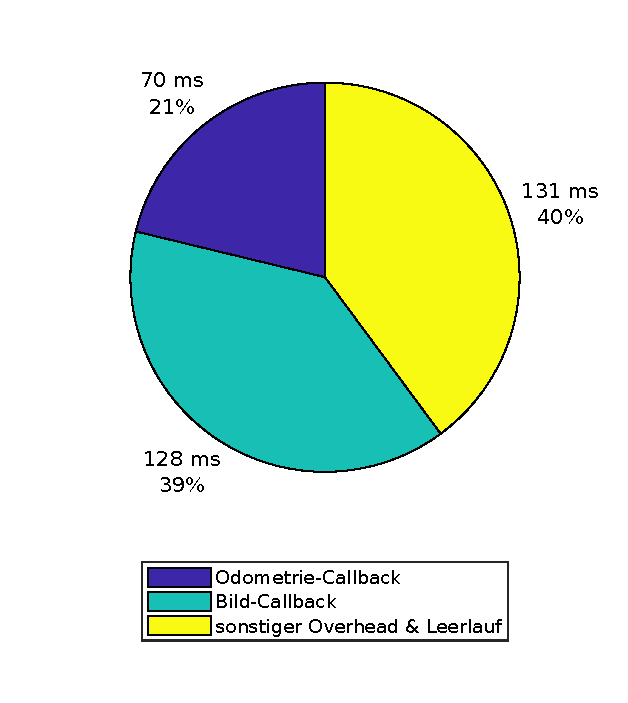
\includegraphics[width=0.7\textwidth]{evaluation_riverflow_times_combined_3Hz_0_2m_s_pie_median}
	\label{fig:evaluation:riverflow:times_combined_3Hz_0_2m_s_pie_median}
	\caption{Zeitbedarf aller Fahrspurverfolgungskomponenten bei \SI{3}{\hertz} Bildfrequenz; Median aller Messwerte einer Runde der Teststrecke}
\end{figure}

\begin{figure}[ht] % [htb]
	\centering
	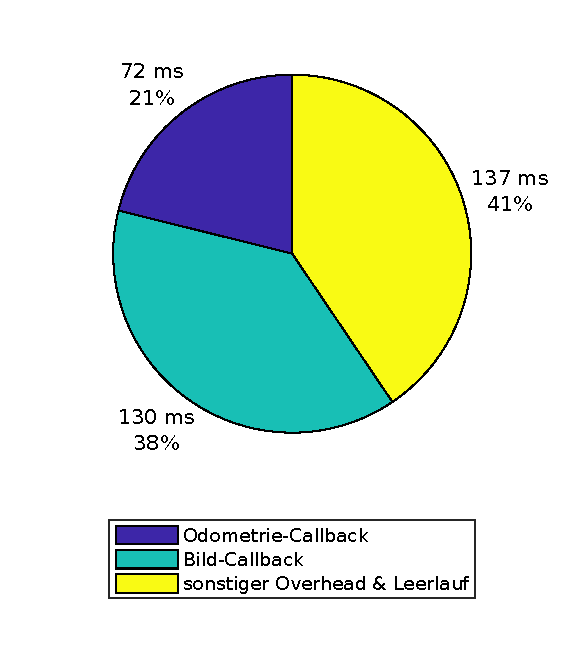
\includegraphics[width=0.7\textwidth]{evaluation_riverflow_times_combined_3Hz_0_2m_s_pie_mean}
	\label{fig:evaluation:riverflow:times_combined_3Hz_0_2m_s_pie_mean}
	\caption{Zeitbedarf aller Fahrspurverfolgungskomponenten bei \SI{3}{\hertz} Bildfrequenz; Mittelwert aller Messwerte einer Runde der Teststrecke}
\end{figure}

\paragraph{Dauer einzelner Komponenten der Fahrspurerkennung}
Um in Zukunft Optimierungen an den implementierten Bildverarbeitungsalgorithmen durchführen zu können ist es unumgänglich nicht nur die gesamt benötigte Zeit, sondern auch die Dauer der einzelnen Module zu messen.

\begin{figure}[ht] % [htb]
	\centering
	\subfloat[Boxplot ohne Startphase\label{fig:evaluation:riverflow:times_pic_3Hz_0_2m_s_boxplot}]{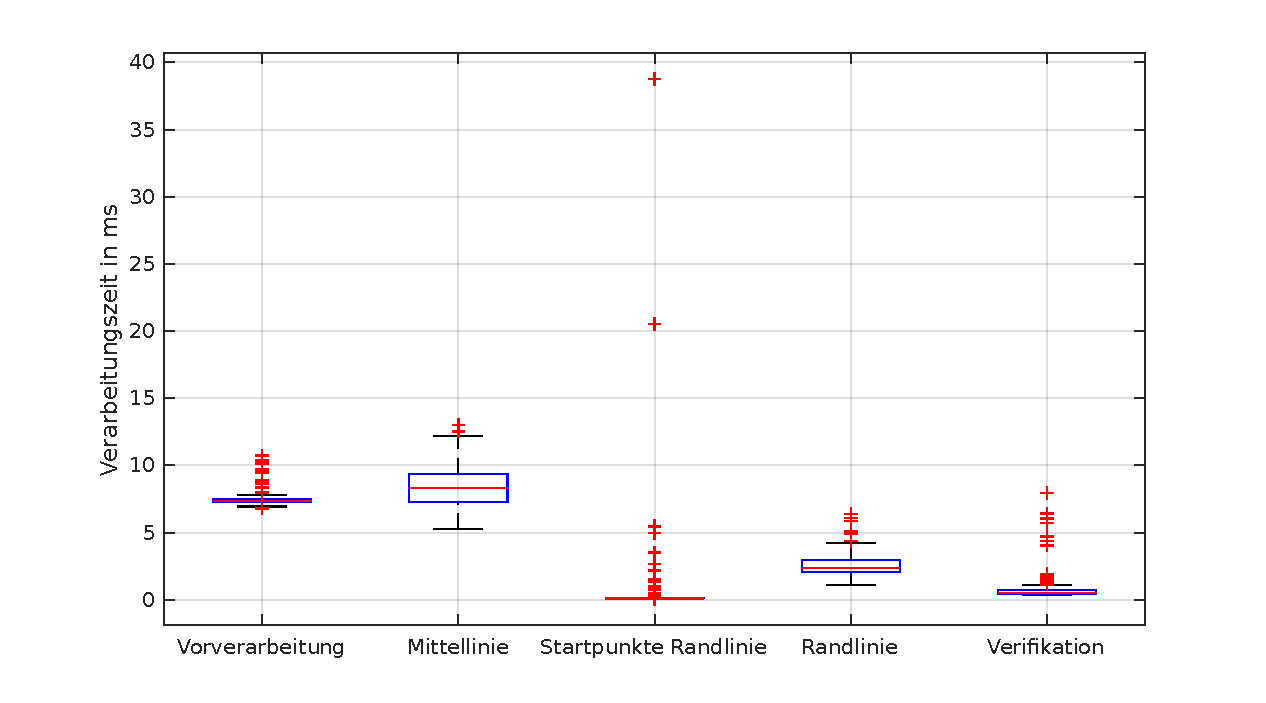
\includegraphics[width=0.7\textwidth]{evaluation_riverflow_times_pic_3Hz_0_2m_s_boxplot}}
	\qquad
	\subfloat[Boxplot ohne Startphase\label{fig:evaluation:riverflow:times_pic_3Hz_0_2m_s_boxplot_ros}]{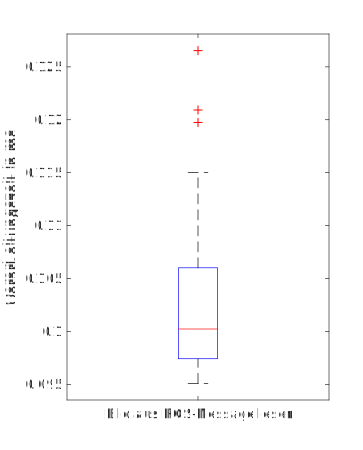
\includegraphics[width=0.2\textwidth]{evaluation_riverflow_times_pic_3Hz_0_2m_s_boxplot_ros}}
	\subfloat[Tortendiagramm; Median aller Messwerte einer Runde\label{fig:evaluation:riverflow:times_pic_3Hz_0_2m_s_pie_no_ros}]{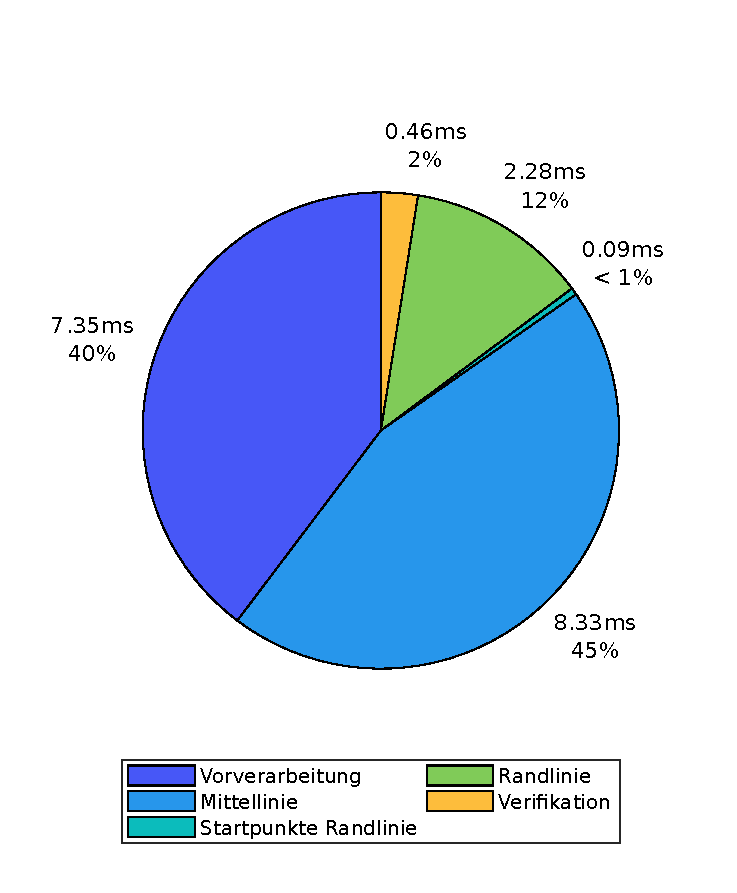
\includegraphics[width=0.45\textwidth]{evaluation_riverflow_times_pic_3Hz_0_2m_s_pie_no_ros}}
	%Summe:18.5185ms
	\qquad
	\subfloat[Tortendiagramm; Median aller Messwerte einer Runde; mit Dekompression des Bildes\label{fig:evaluation:riverflow:times_pic_3Hz_0_2m_s_pie_with_ros}]{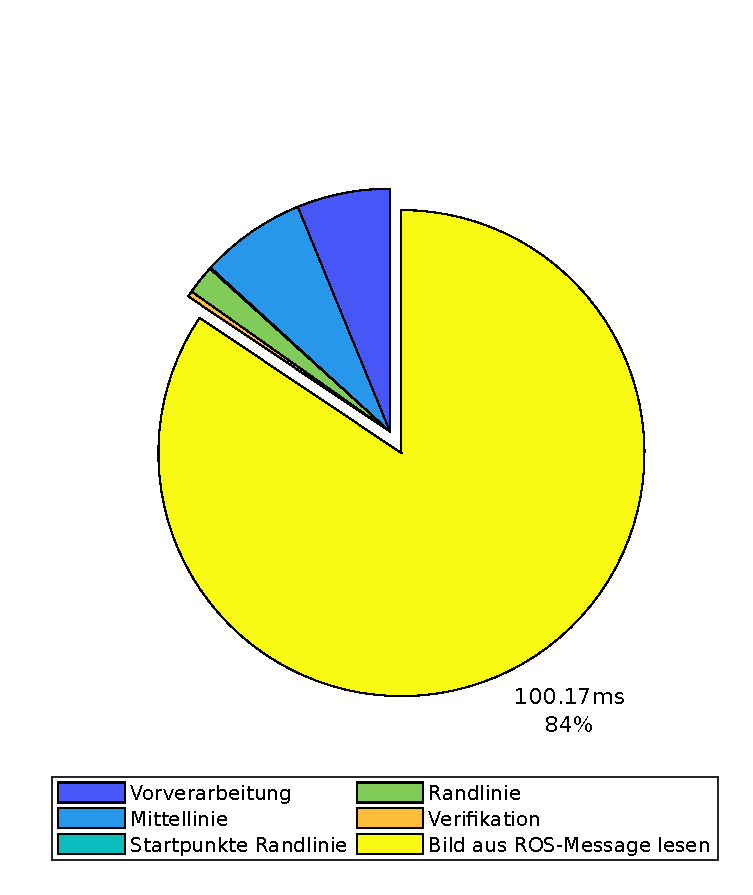
\includegraphics[width=0.45\textwidth]{evaluation_riverflow_times_pic_3Hz_0_2m_s_pie_with_ros}}
	\caption{Zeitbedarf aller Fahrspurerkennungskomponenten bei \SI{3}{\hertz} Bildfrequenz}
\end{figure}

Diese Untersuchungen führten zu interessanten Ergebnissen, welche die Echtzeitfähigkeit der MATLAB-\gls{acr:ros}-Schnittstelle in Frage stellen. Wie in Abbildung \ref{fig:evaluation:riverflow:times_pic_3Hz_0_2m_s_pie_with_ros} zu sehen, wird ein Großteil der Dauer eines Bild-Callbacks zum Umwandeln der \gls{acr:ros}-Message in eine von MATLAB prozessierbare Matrix benötigt. Eine genauere Untersuchung mit dem MATLAB-Profiler zeigte, dass in diesem Schritt eine Dekompression des im JPEG-Format übertragenen Bildes den wesentlichen Anteil dieses Zeitbedarfs verursacht. Eine unkomprimierte Übertragung würde jedoch ein vielfaches dieser Dauer in Anspruch nehmen.

Der eigens entwickelte Anteil der Fahrspurerkennung benötigt im Median einer Runde lediglich \SI{18,5}{ms}, die genaue Aufteilung kann in Abb. \ref{fig:evaluation:riverflow:times_pic_3Hz_0_2m_s_pie_no_ros} sowie \ref{fig:evaluation:riverflow:times_pic_3Hz_0_2m_s_boxplot} nachvollzogen werden. Die meiste Zeit wird für Bildvorverarbeitung und Mittellinienerkennung benötigt. Da diese Funktionen zum Großteil auf vorgegebenen, komplexen und bereits maschinennah implementierten MATLAB-Funktionen basieren, kann hier nur unter Nutzung anderer Software eine Optimierung stattfinden. Die zum Großteil aus elementaren Funktionen aufgebaute Erkennung\&Verifikation der Randlinie läuft schon erfreulich schnell ab, sodass hier trotz der vielen verwendeten, in MATLAB rechenzeitintensiven Schleifen keine zügigere Alternative gesucht werden muss.

\subparagraph{Startpunktfindung}
Wie in Abb. \ref{fig:evaluation:riverflow:times_pic_3Hz_0_2m_s_pie_no_ros} zu sehen, verstreicht im Normalfall bei der Feststellung der Startpunkte zur Erkennung der seitlichen Fahrbahnmarkierungen kaum Zeit. Wird jedoch kein Mittellinienelement nahe genug vor dem Fahrzeug gefunden, so gestaltet sich dieser Prozess aufwendiger (siehe Abschnitt \ref{sssec:fahrspurerkennung:riverflow:randlinie:startpunktgewinnung}). Abbildung \ref{fig:evaluation:riverflow:times_startpoints_3Hz_0_2m_s_boxplot} gibt ein besseres Bild der Messwerte wieder als Diagramm \ref{fig:evaluation:riverflow:times_pic_3Hz_0_2m_s_pie_no_ros} bzw. \ref{fig:evaluation:riverflow:times_pic_3Hz_0_2m_s_boxplot}, da hier nicht nur der Median aller Messwerte gebildet, sondern vor der Erstellung des Boxplots die Daten nach Art der Methode zur Startpunktbestimmung sortiert werden. 
\begin{figure}[ht] % [htb]
	\centering
	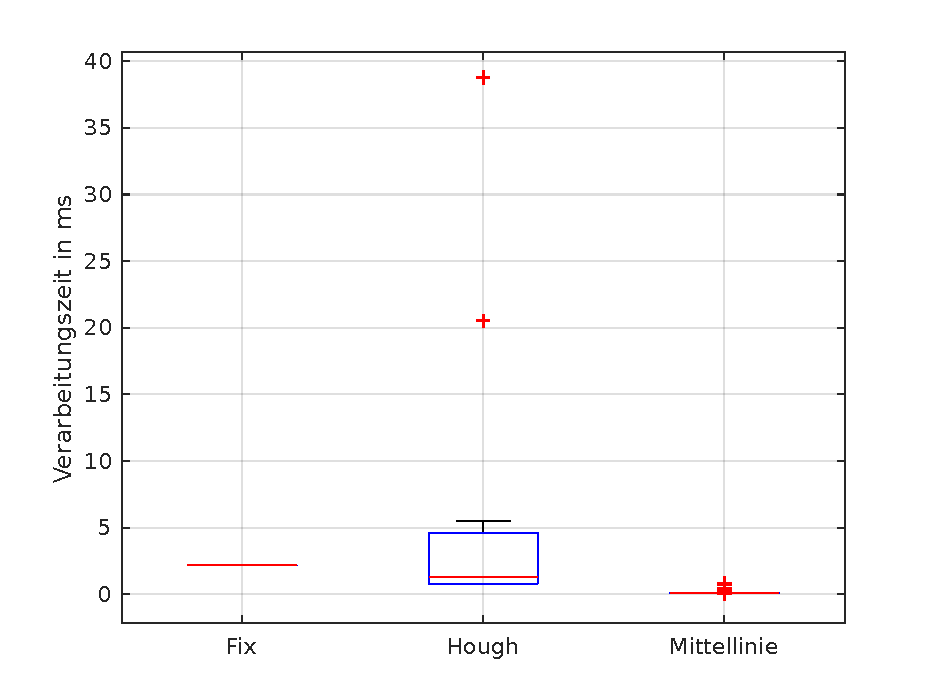
\includegraphics[width=0.7\textwidth]{evaluation_riverflow_times_startpoints_3Hz_0_2m_s_boxplot}
	\label{fig:evaluation:riverflow:times_startpoints_3Hz_0_2m_s_boxplot}
	\caption{Zeitbedarf der Startpunktfindungsalgorithmen für die Erkennung der seitlichen Fahrbahnmarkierungen bei \SI{3}{\hertz} Bildfrequenz}
\end{figure}
Die Erwartung, dass bei Nutzung der mittigen Fahrbahnmarkierung zu Startpunktgenerierung kaum Zeit vergeht, wurde durch den über diese Kategorie gebildeten Median von \SI{0,09}{ms} bestätigt. Jedoch ist auch die von der eindimensionalen Hough-Transformation benötigte Laufzeit von \SI{1,32}{ms} vertretbar. Die In Abbildung \ref{fig:evaluation:riverflow:times_startpoints_3Hz_0_2m_s_boxplot} sichtbaren Ausreißer entstehen durch das erstmalige ausführen der Funktion, welche nicht während der im Boxplot unberücksichtigten \glqq Warmlaufphase\grqq\ geschieht. Da nur einmal fix im Bildkoordinatensystem liegende Punkte genutzt werden mussten und dieser Fall nur nach Fehlschlag der eindimensionalen Hough-Transformation auftritt, wird dieser Messwert nur als Median ohne Box etc. in Abb. \ref{fig:evaluation:riverflow:times_startpoints_3Hz_0_2m_s_boxplot} dargestellt und bewegt sich mit \SI{2,17}{ms} im Bereich dieser Methode.

\paragraph{Übertragungszeit}
Die Übertragungszeit der Bilder von \SI{77,2}{ms} im Median stellt eine erhebliche Totzeit dar. Die Streuung dieser bis hin zu \SI{183}{ms} spiegelt die Probleme der Nutzung einer WLAN-Verbindung, welche gern zu unvorhersehbaren Latenzen neigt, wieder. Durch eine JPEG-Kompression mit einer Qualitätseinstellung von 20\% wurde der Bildtransfer schon signifikant beschleunigt.

\begin{figure}[ht] % [htb]
	\centering
	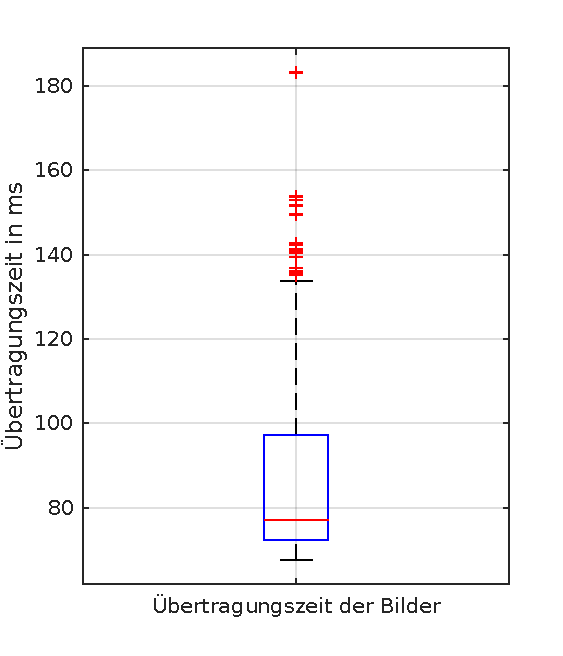
\includegraphics[width=0.7\textwidth]{evaluation_riverflow_times_pictransfer_3Hz_0_2m_s_boxplot}
	\label{fig:evaluation:riverflow:times_pictransfer_3Hz_0_2m_s_boxplot}
	\caption{Übertragungszeit der Aufnahmen bei \SI{3}{\hertz} Bildfrequenz}
\end{figure}

\section{Geschwindigkeit \dcfirstauthorshort}
\label{ssec:evaluation:messungen:geschwindigkeit}
%In diesem Abschnitt soll untersucht werden, ob eine Reduzierung der Geschwindigkeit positive Auswirkungen auf die Zuverlässigkeit von Bildverarbeitung und Regelung besitzt.

Nachdem eine passende Einstellung der Regel-und Bildverarbeitungsfrequenz gefunden wurde, soll nun das Fahren mit höheren Geschwindigkeiten betrachtet werden. Neben der Sichtprüfung der Funktionalität der Fahrspurverfolgung wurden die Anzahl der zur Zielpunktbestimmung genutzten Punkte pro Regelungsiteration und der prozentuale Anteil an nicht bestimmten Zielpunkten zur Untersuchung herangezogen. 

Zur besseren Vergleichbarkeit der Messergebnisse wurden die Daten für je eine entgegen des Uhrzeigersinnes gefahrene Runde mit \SI{3}{\hertz} Bildverarbeitungsfrequenz aufgenommen.

Abbildung~\ref{fig:evaluation:riverflow:regelungspunkte:je_linie} zeigt exemplarisch für die Geschwindigkeit \( \gls{lat:velocity} = 
\SI{0,2}{\metre\per\second} \) die  Anzahl jeweiliger Linienpunkttypen zur Zielpunktberechnung. Es fällt sogleich auf, dass die Mittellinie einen kleineren Einfluss nimmt. Da pro Strich und Bild nur ein Punkt in der Weltkarte 
eingetragen wird, ist deren Punkteanzahl geringer. Wie unter 
\ref{item:regelung:zielpunkt:holen:regeln:xcoord} in Kapitel 
\ref{ssec:regelung:zielpunkt:holen} beschrieben, werden die Regelungspunkte unter anderem nach ihrer x-Koordinate ausgewählt. In einer Linkskurve fallen dadurch mehr Punkte der linken Randlinie in das Suchfenster. Da die Strecke in 
der befahrenen Richtung vorrangig Linkskurven aufweist, werden im Mittel mehr linke als rechte Randpunkte zur Zielpunktberechnung herangezogen.

\begin{figure}[htbp] % [htb]
	\centering
	\subfloat[Anzahl der jeweiligen zur Regelung genutzten Punkte aus der Weltkarte bei \( \gls{lat:velocity} = \SI{0,2}{\metre\per\second} \) 
	\label{fig:evaluation:riverflow:regelungspunkte:je_linie}]{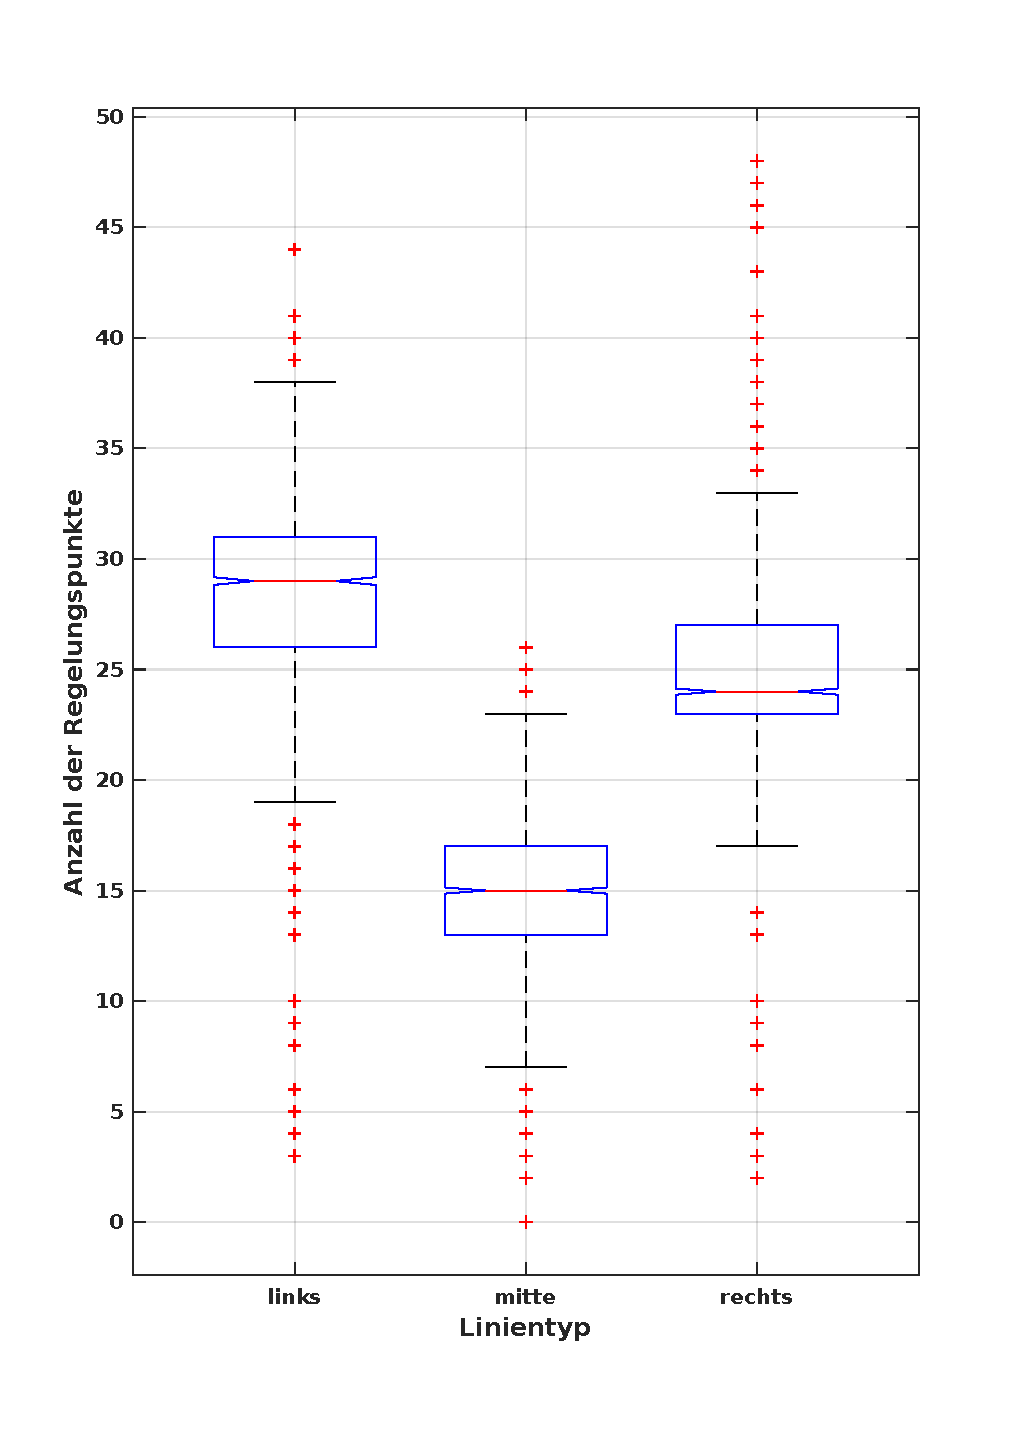
\includegraphics[height=0.35\textheight]{evaluation_riverflow_regelungspunkte_je_linie_0_2m_s_3Hz.pdf}}
	\hfill
	\subfloat[Anzahl der zur Regelung verwendeten Kartenpunkte zu verschiedenen 
	Geschwindigkeiten
	\label{fig:evaluation:riverflow:regelungspunkte:je_geschw}]{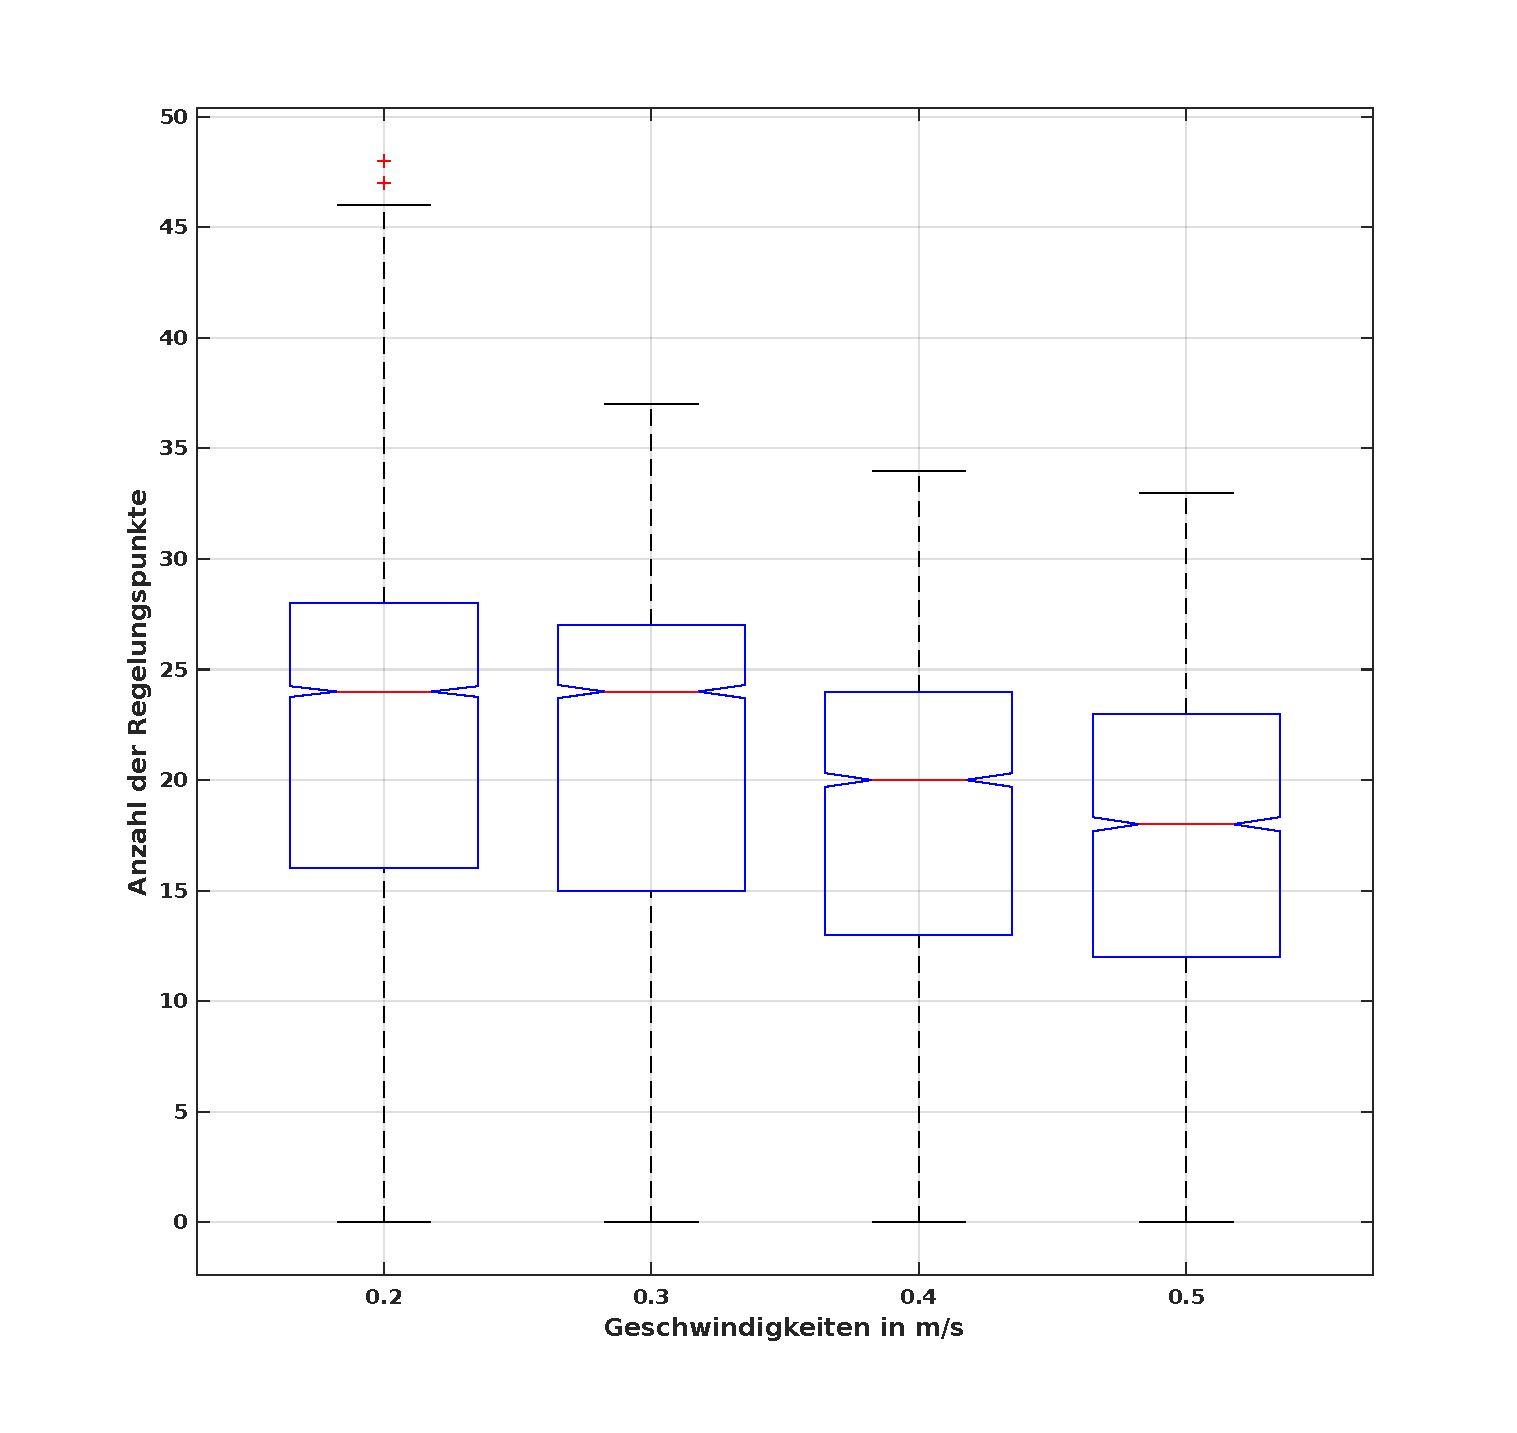
\includegraphics[height=0.35\textheight]{evaluation_riverflow_regelungspunkte_je_geschw_3Hz.pdf}}
	\caption{Boxplots zur Menge der Punkte, welche in einem Regelungsintervall 
	aus der Weltkarte entnommen und zur Zielpunktberechnung verwendet werden}
	\label{fig:evaluation:riverflow:regelungspunkte}
\end{figure}

Betrachten wir die Gesamtzahl der zur Regelung verwendeten Punkte, ist wie in 
Abbildung~\ref{fig:evaluation:riverflow:regelungspunkte:je_geschw} ein Abfallen der Anzahl mit ansteigender Geschwindigkeit des Fahrzeugs zu beobachten. Wenn das Auto schneller fährt, liegt ein Punkt in der Karte umso eher außerhalb des Bereiches, aus dem die Regelungspunkte genutzt werden. Bei gleichbleibender Bildfrequenz wird zwischen jedem Bild eine größere Strecke zurückgelegt, sodass die Dichte der Weltkartenpunkte geringer wird. Der dargestellte Boxplot erfüllt also die Erwartungen.

Die mit unserer Implementierung erreichbare Höchstgeschwindigkeit sollte folglich dann erreicht sein, wenn der mobile Roboter fast ausschließlich nach den Informationen eines Bildes regelt oder sogar zwischenzeitlich keine Zielpunkte mangels Regelungspunkten bestimmen kann. Mit anderen Worten: Wenn sich das Auto zwischen zwei Aufnahmen bis zum Sichtende des ersten Bildes bewegt, wie der Riverflow-Algorithmus Punkte erkennen konnte, ist die Maximalgeschwindigkeit beinahe erreicht. Ein Indiz dafür ist neben der visuellen Auffälligkeit des Fahrspurverlasses die starke Zunahme der nicht gefundenen Zielpunkte. 

\begin{figure}[htbp] % [htb]
	\centering
	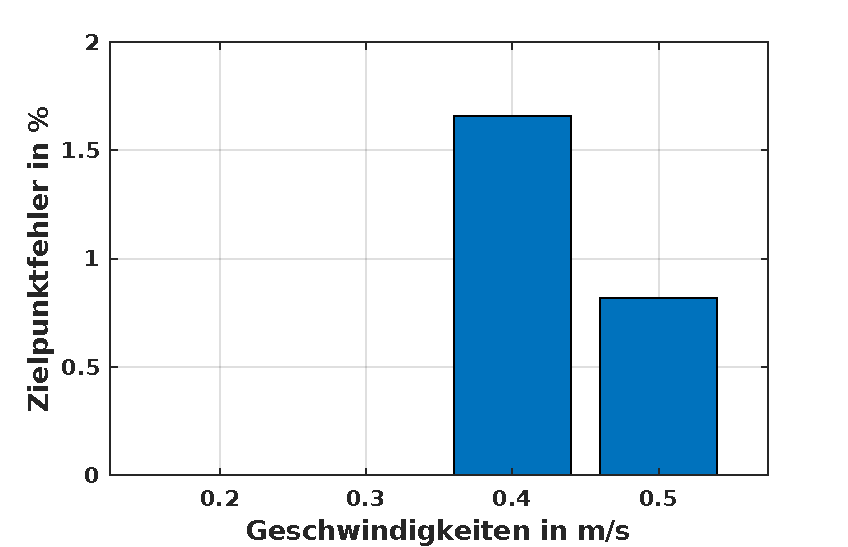
\includegraphics[width=0.7\textwidth]{evaluation_riverflow_zielpunktfehler_je_geschw_3Hz.pdf}
	\caption{Anteil der unbestimmten Zielpunkte einer Runde auf dem Parcours mit verschiedenen Geschwindigkeiten}
	\label{fig:evaluation:riverflow:zielpunktfehler_je_geschw}
\end{figure}

Was in Abbildung~\ref{fig:evaluation:riverflow:zielpunktfehler_je_geschw} zu sehen ist, war ebenfalls während des Fahrversuches am Auto zu beobachten. Ab einer Geschwindigkeit von \( \gls{lat:velocity} = \SI{0,4}{\metre\per\second} \) fuhr das Fahrzeug instabiler und die Latenzzeit der Regelung war dahingehend zu bemerken, dass in Kurven meist etwas zu spät und kurz darauf zur Korrektur zu viel eingelenkt wurde. Dies führte zu einer schwingenden Fahrweise (das Auto fuhr \glqq Schlängellinien\grqq). 

Die begrenzende Komponente für die Geschwindigkeit ist hier neben der Bildfrequenz allerdings auch das Getriebe. Durch dessen kurze Übersetzung beträgt die Geschwindigkeit im Maximum 4500 tics pro Sekunde, was in etwa \SI{0,43}{\metre\per\second} entspricht. Die im Plot bezeichneten \SI{0,5}{\metre\per\second} dürften folglich nicht genau stimmen, auch wenn dies der eingestellte Wert des Geschwindigkeitsparameters war. Sie geben die Daten zu der dem ersten Auto maximal physikalisch möglichen Geschwindigkeit an. 

Ergänzend muss hier erwähnt werden, dass bereits ein zweites Fahrzeug mit ca. doppelt so langer Übersetzung existiert. Jedoch misslang eine Testfahrt mit unveränderten Parametereinstellungen bei höheren Geschwindigkeiten. Auch hier zeigte sich die Grenze an der \SI{0,5}{\metre\per\second}-Marke.

Dass diese Geschwindigkeit auch die Grenze der Stabilität des Algorithmus war, zeigte ein \glqq Dauertest\grqq{} von zehn Runden. Bis zu einer Geschwindigkeit von \SI{0,3}{\metre\per\second} führte der Versuch zu keinen nennenswerten Problemen in der Fahrspurverfolgung. Auch wenn während der schnelleren \SI{0,4}{\metre\per\second}-Fahrt zehn Runden erfolgreich abgefahren wurden, kam hier das Fahrzeug mitunter stark ins Schwingen und befand sich kurz davor, den Fahrstreifen zu verlieren. Mit der höchstmöglichen Geschwindigkeit wurde der Dauertest nicht bestanden, da das Auto schon nach zwei Runden von der Straße abkam.
\subsection{Hinzufügen von Objekten zum Testszenario \dcsecondauthorshort}
\label{ssec:evaluation:messungen:objekte_hinzufuegen}
Im realen Straßenverkehr befinden sich in der Regel mehr Objekte im Sichtbereich des Fahrers bzw. der Kamera als die bis jetzt im Parcours alleinig vorhandenen Fahrbahnmarkierungen. Diese Gegenstände können für die Trajektorieplanung relevant sein (Hindernisse) oder in keinem Zusammenhang damit stehen (Objekte abseits der Straße). Da der bis jetzt implementierte Fahrspurverfolgungsalgorithmus keine Hinderniserkennung und -vermeidung besitzt, kann hier nur auf Gegenstände neben der Fahrspur eingegangen werden. In diesem Abschnitt sollen Untersuchungen stattfinden, ob die Erkennung des Straßenverlaufs auch bei Hinzufügen weiterer Gegenstände zum Testszenario noch zufriedenstellend abläuft.

\paragraph{Betrachtungen zur Bildvorverarbeitung}
\label{par:evaluation:riverflow:messungen:objekte_hinzufuegen}
Vor der Durchführung von Testfahrten muss die Frage gestellt werden, wann dem Parcours hinzugefügte Elemente einen Einfluss auf die Fahrspurerkennung haben können. Da die Filterung und anschließende Binarisierung des entzerrten Graustufenbildes den Ausgangspunkt für darauffolgende Programmkomponenten darstellen, muss das Objekt die \glqq Hürde\grqq\ dieser Informationsreduktion überwinden können. Konkret bedeutet dies, dass sein Kontrast im Vergleich zum umliegenden Szenario groß genug sein muss, um als schwellwertüberschreitende Filterantwort des Kantendetektors im Binärbild aufzutreten oder als relevantes Maxima auf einer Scanline gefunden zu werden (s. Abschnitt \ref{sec:bildvorverarbeitung:binarisierung} bzw. \ref{ssec:fahrspurerkennung:kalman:messung}).
Als Vorversuch wurden farbige Blätter (Abb. \ref{fig:evaluation:riverflow:test_kontraste_roh}) verschiedener Helligkeit (Abb. \ref{fig:evaluation:riverflow:test_kontraste_entzerrt}) im Testszenario platziert. Abbildung \ref{fig:evaluation:riverflow:test_kontraste_gefiltert} zeigt wie erwartet, dass nur sehr dunkle Farben eine ausreichend große Filterantwort hervorrufen, welche im Binärbild (Abb. \ref{fig:evaluation:riverflow:test_kontraste_binarisiert}) als Kante vermerkt wird. Auffällig ist auch, dass die Eckpunkte der Blätter eine besonders große Filterantwort bewirken, die eigentlichen Kanten aber nur beim roten (teilweise) und schwarzen Blatt erkannt werden.

\begin{figure}[htbp] % [htb]
%\centering
%\hfill
\subfloat[roh\label{fig:evaluation:riverflow:test_kontraste_roh}]{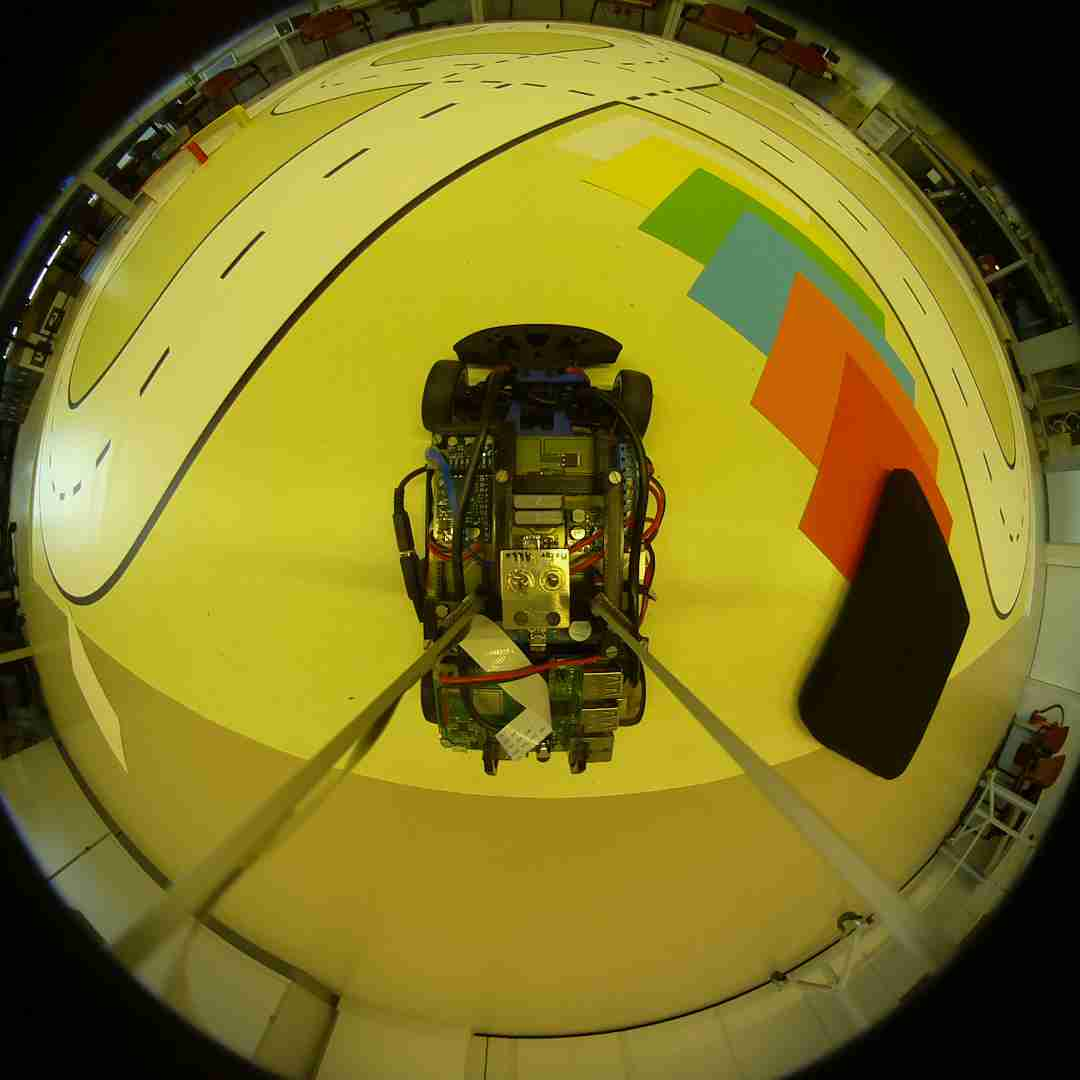
\includegraphics[width=0.49\textwidth]{evaluation_riverflow_test_kontraste_roh}}
\hfill
\subfloat[entzerrt\label{fig:evaluation:riverflow:test_kontraste_entzerrt}]{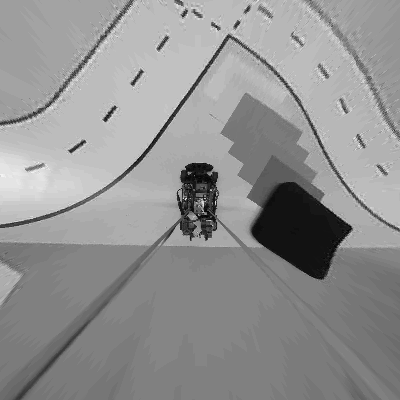
\includegraphics[width=0.49\textwidth]{evaluation_riverflow_test_kontraste_entzerrt}}
\hfill
\subfloat[gefiltert\label{fig:evaluation:riverflow:test_kontraste_gefiltert}]{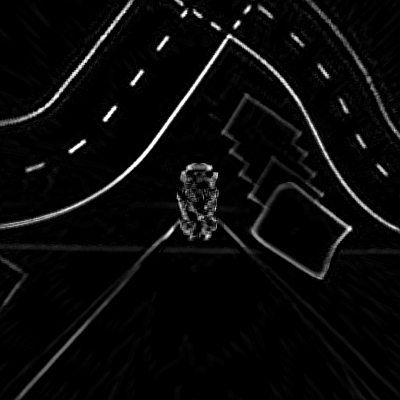
\includegraphics[width=0.49\textwidth]{evaluation_riverflow_test_kontraste_gefiltert}}
\hfill
\subfloat[binarisiert\label{fig:evaluation:riverflow:test_kontraste_binarisiert}]{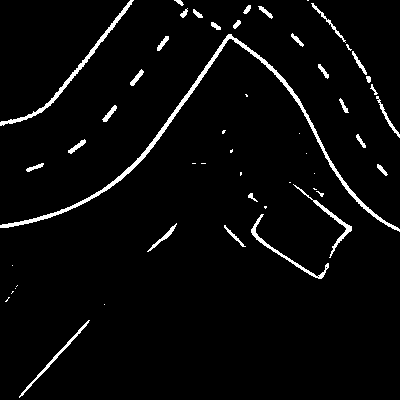
\includegraphics[width=0.49\textwidth]{evaluation_riverflow_test_kontraste_binarisiert}}
%\hfill
\label{fig:evaluation:riverflow:test_kontraste}
\caption{Vorversuch Kontraste zusätzlicher Objekte im Testszenario}
\end{figure}

\paragraph{Objekte neben der Fahrspur}
Es wurden einige Quader, in den Farben des in Abschnitt \ref{par:evaluation:riverflow:messungen:objekte_hinzufuegen} untersuchten Papiers, im Parcours positioniert (s. Abb. \ref{fig:evaluation:riverflow:test_kontraste_versuchsaufbau_haeuser}). Hierbei wurde bei 3 Fahrten der Abstand zur seitlichen Fahrbahnmarkierung von \SI{16}{cm} (größer der Länge einer Scanline) über \SI{4}{cm} (kleiner der Länge einer Scanline) hin zu \SI{0}{cm} verändert.

Können die Scanlines die Kanten eines solchen Objektes nicht erreichen, so ist kein Einfluss auf die Erkennung der Randlinien zu erwarten. Ist der Kontrast eines Quaders zur hellgrünen Grundfarbe des Testszenarios zu gering, so ist eine Fehldetektion aufgrund dessen ebenfalls ausgeschlossen. Eventuelle Beeinträchtigungen des Riverflow-Algorithmus sind somit nur bei den Versuchen mit \SI{4}{cm} und \SI{0}{cm} Abstand bei dunklen Farben der \glqq Störobjekte \grqq\ zu erwarten.

Der Roboter fuhr jedoch auch in diesen Konstellationen fehlerfrei die Runde. Es konnten bei allen Testfahrten keine falsch in der Weltkarte eingetragenen Punkte identifiziert werden.
 
\begin{figure}[htbp] % [htb]
\centering
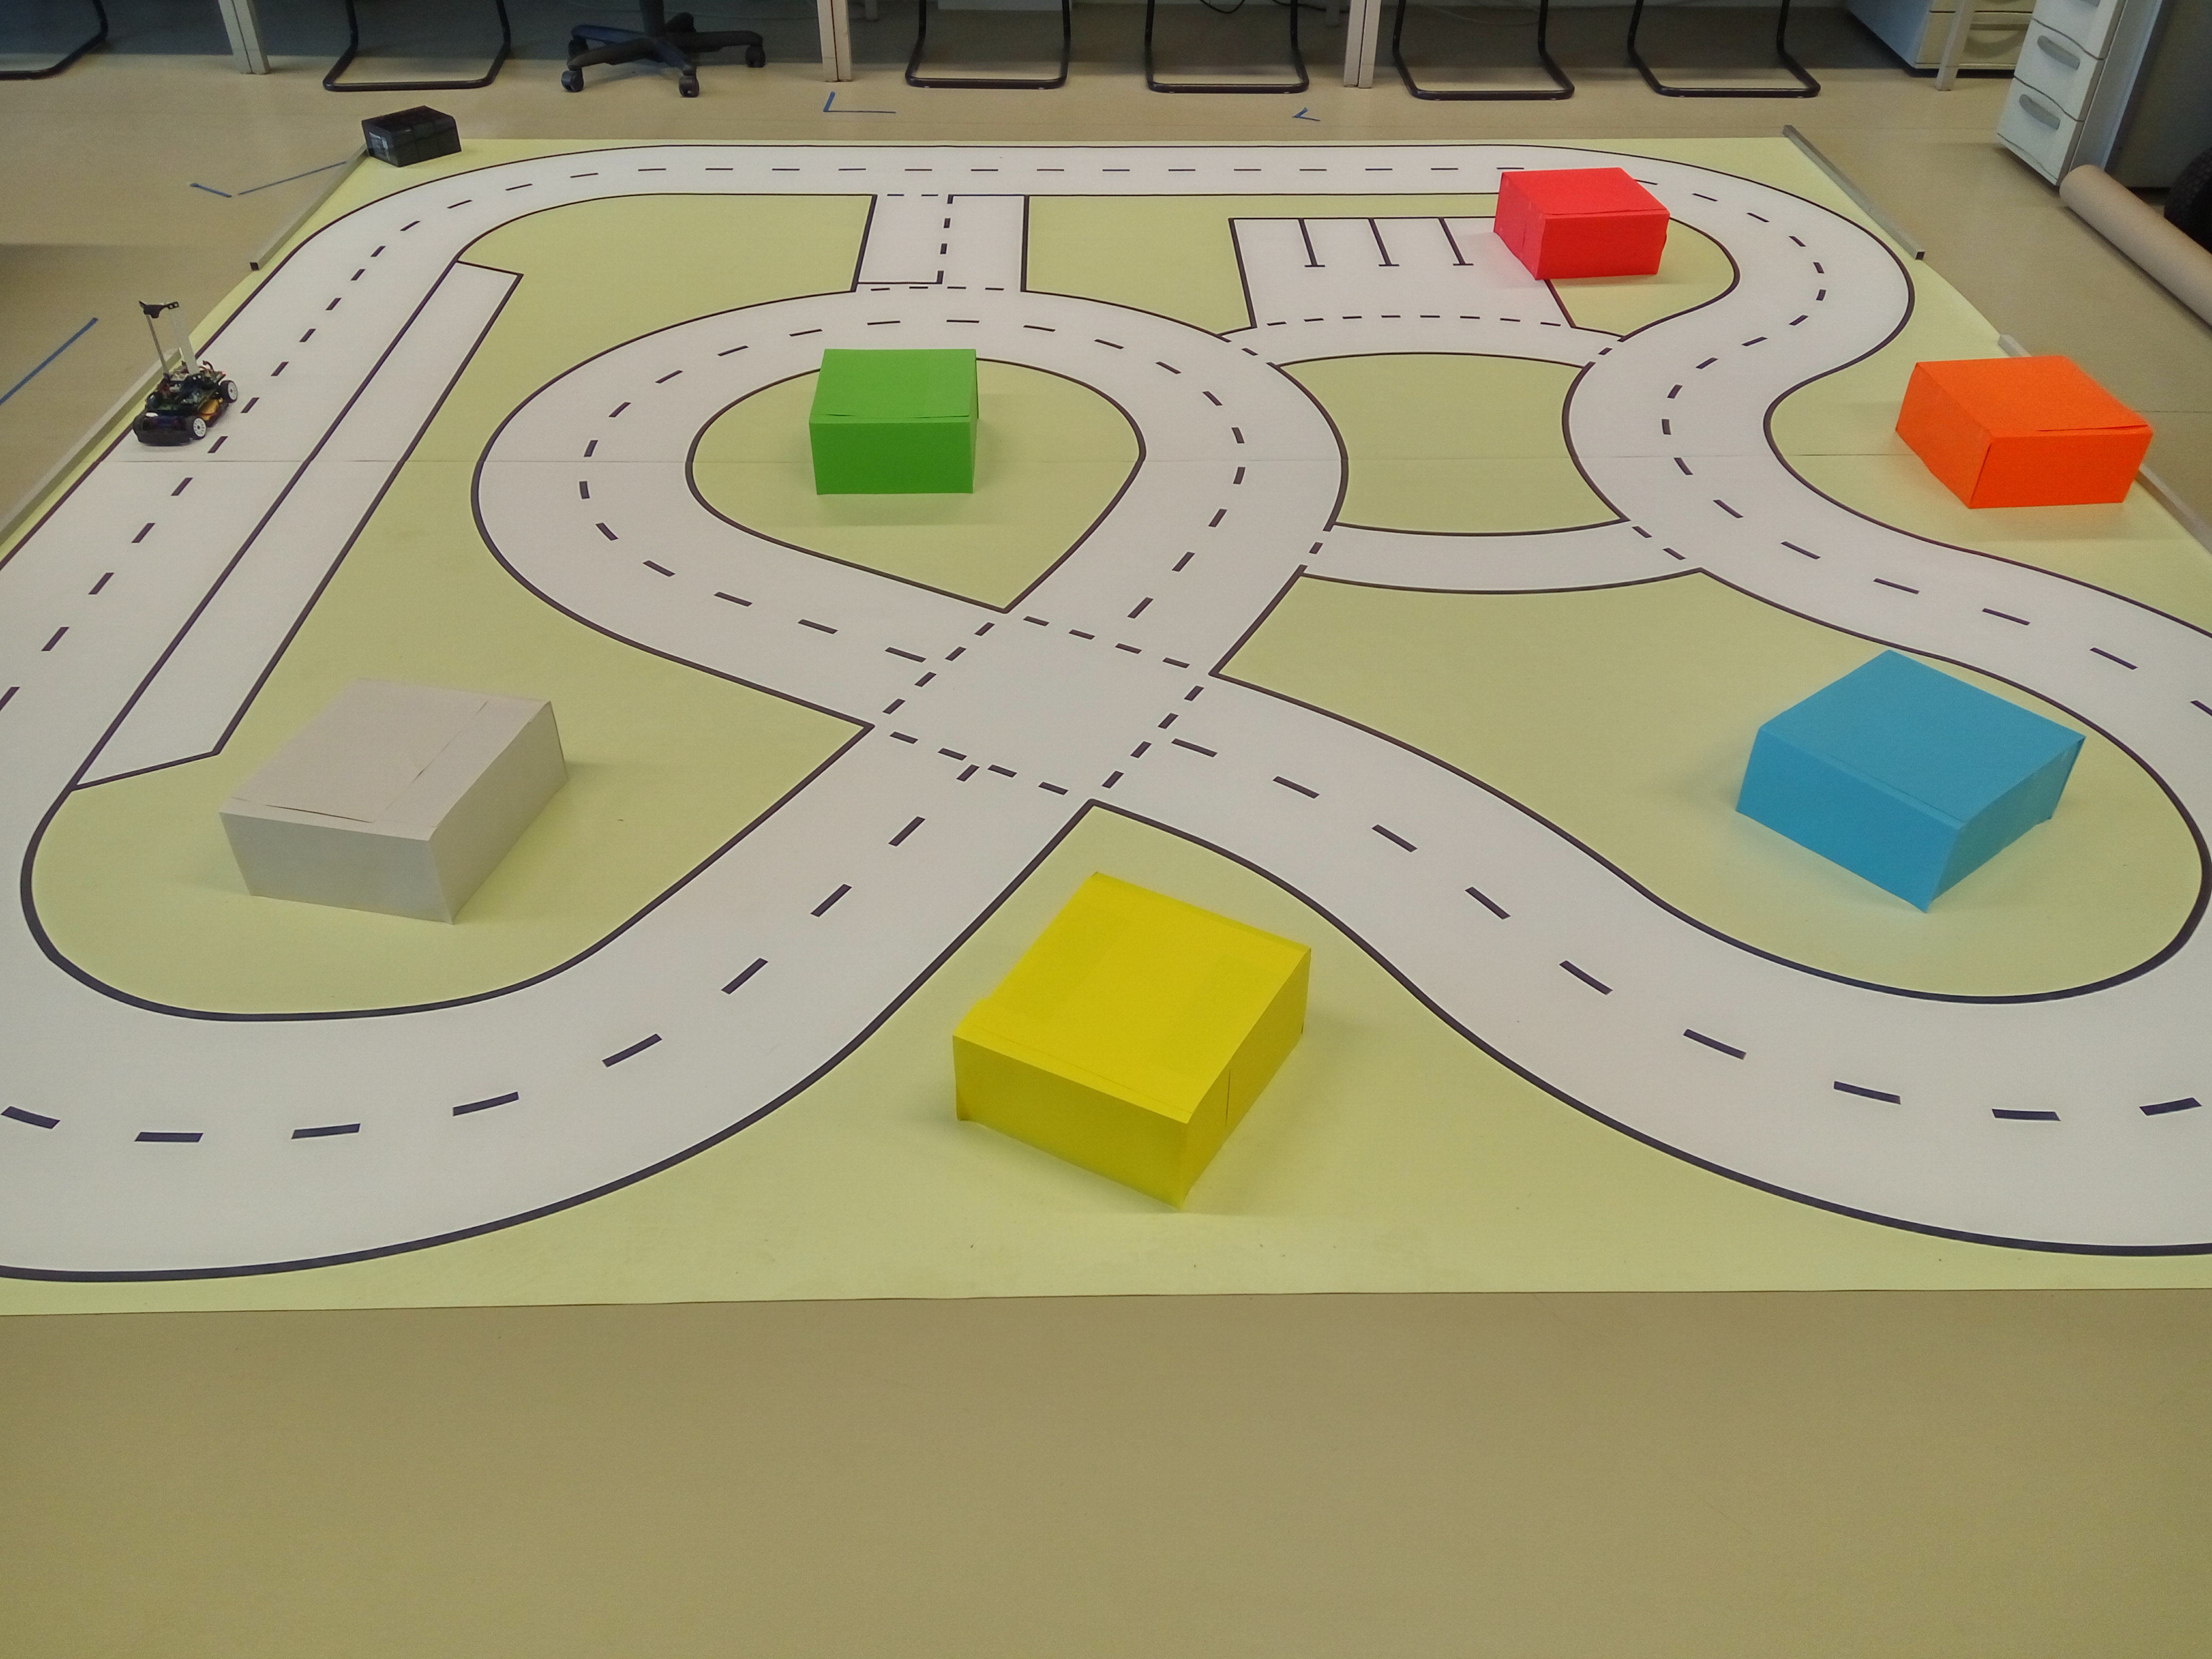
\includegraphics[width=0.5\textwidth]{evaluation_riverflow_test_kontraste_versuchsaufbau_haeuser}
\caption{Versuchsaufbau farbige Quader im Testszenario}
\label{fig:evaluation:riverflow:test_kontraste_versuchsaufbau_haeuser}
\end{figure}

Diese Robustheit gegenüber den hinzugefügten Quadern wurde auf die Verifikation der Punkte nach der Erkennung zurückgeführt, somit soll nun noch die Performanz des Algorithmus ohne diese Komponente betrachtet werden. Charakteristisch für eine Beeinträchtigung an dieser Stelle wäre das Anlegen vieler Hypothesen (möglicher Verläufe der Randlinien), da auf einer Scanline mehrere potentielle zentral auf einer Fahrbahnmarkierung gelegenen Punkte gefunden werden (s. Abschnitt \ref{sssec:fahrspurerkennung:riverflow:randlinie:zentraler_algorithmus}).
\begin{figure}[htbp] % [htb]
%\centering
%\hfill
\subfloat[keine \glqq Störobjekte\grqq \label{fig:evaluation:riverflow:hypos_hist_inf}]{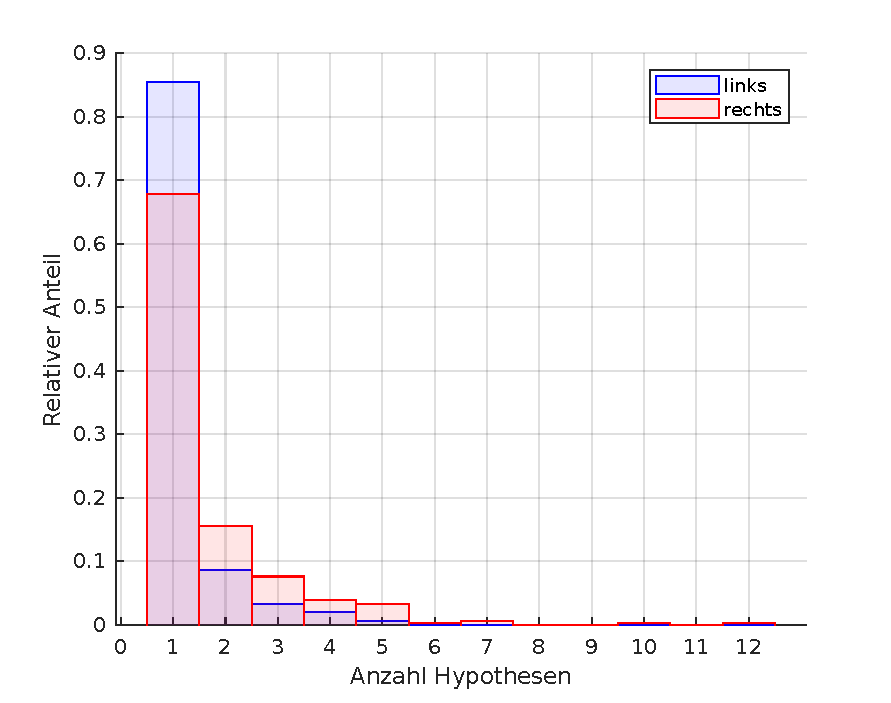
\includegraphics[scale=\mtlstscale]{evaluation_riverflow_hypos_hist_inf}}
\hfill
\subfloat[\SI{16}{cm}\label{fig:evaluation:riverflow:hypos_hist_16}]{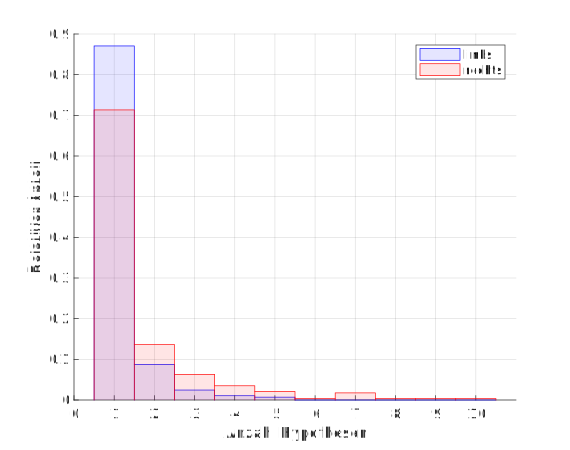
\includegraphics[scale=\mtlstscale]{evaluation_riverflow_hypos_hist_16}}
\hfill
\subfloat[\SI{4}{cm}\label{fig:evaluation:riverflow:hypos_hist_04}]{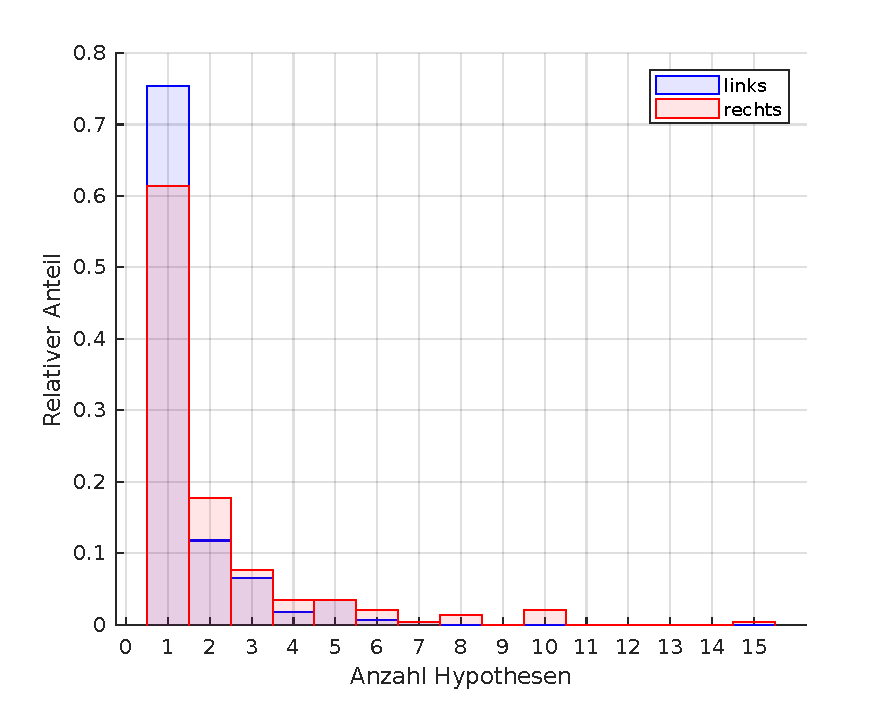
\includegraphics[scale=\mtlstscale]{evaluation_riverflow_hypos_hist_04}}
\hfill
\subfloat[\SI{0}{cm}\label{fig:evaluation:riverflow:hypos_hist_00}]{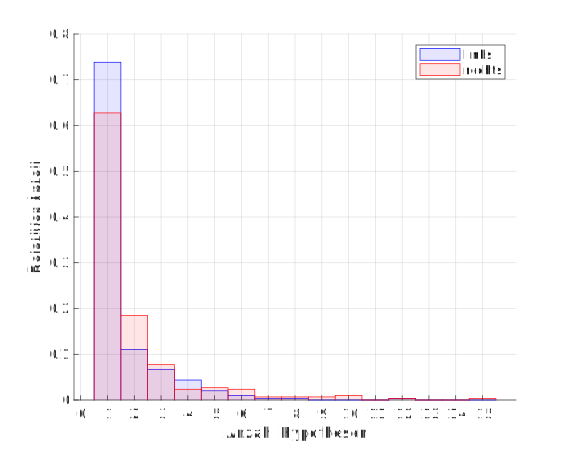
\includegraphics[scale=\mtlstscale]{evaluation_riverflow_hypos_hist_00}}
%\hfill
\caption{Histogramme Hypothesenanzahl mit \glqq Störobjekten\grqq\ im Testszenario; Variation des Abstandes von der Fahrspur}
\label{fig:evaluation:riverflow:hypos_hists}
\end{figure}

Abbildung \ref{fig:evaluation:riverflow:hypos_hists} bestätigt diese Vermutung, es ist ein häufigeres Auftreten mehrerer Hypothesen für die seitlichen Fahrbahnmarkierungen zu beobachten, wenn diese in die von den Scanlines aufgespannten \gls{acr:roi}'s platziert werden. Beispiele für diese Fehlerkennungen sind in Abbildung \ref{fig:evaluation:riverflow:hypos_riverflow_plots} zu sehen.
\begin{figure}[htbp] % [htb]
%\centering
%\hfill
\subfloat[\label{fig:evaluation:riverflow:hypos_riverflow_plot_1}]{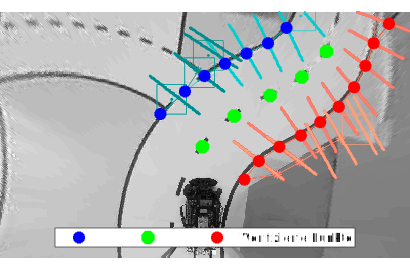
\includegraphics[width=0.49\textwidth]{evaluation_riverflow_hypos_riverflow_plot_1}}
\hfill
\subfloat[\label{fig:evaluation:riverflow:hypos_riverflow_plot_2}]{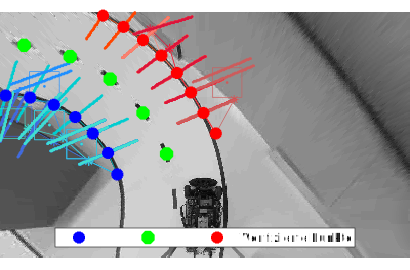
\includegraphics[width=0.49\textwidth]{evaluation_riverflow_hypos_riverflow_plot_2}}
\hfill
\subfloat[\label{fig:evaluation:riverflow:hypos_riverflow_plot_3}]{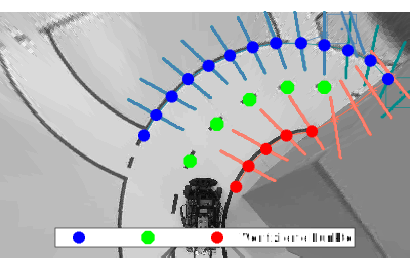
\includegraphics[width=0.49\textwidth]{evaluation_riverflow_hypos_riverflow_plot_3}}
\hfill
\subfloat[\label{fig:evaluation:riverflow:hypos_riverflow_plot_4}]{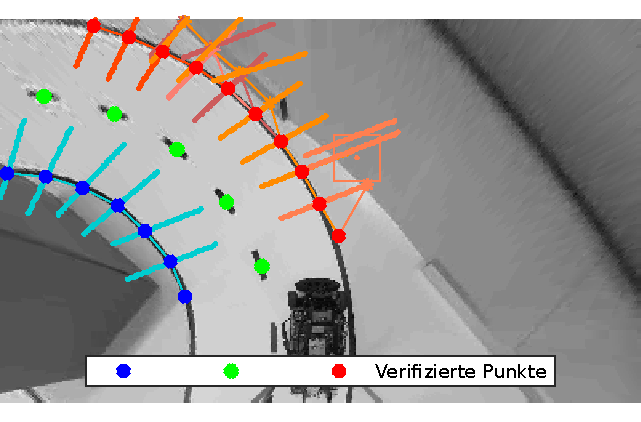
\includegraphics[width=0.49\textwidth]{evaluation_riverflow_hypos_riverflow_plot_4}}
%\hfill
\caption{Beispiele für die Erkennung mehrerer Hypothesen mit \glqq Störobjekten\grqq\ im Testszenario}
\label{fig:evaluation:riverflow:hypos_riverflow_plots}
\end{figure}

Ein weiterer Grund für die Detektion mehrerer möglicher Verläufe der Randlinie stellt, wie in Abbildung \ref{fig:evaluation:riverflow:hypos_riverflow_plot_4} zu sehen, die Erkennung schon immer im Testszenario vorhandener, bis jetzt nicht weiter berücksichtigter Kanten dar. Die Ränder der PVC-Plane, auf welche die Strecke gedruckt wurde oder die zum Beschweren dieser genutzten Alu-Profile sind häufig die Ursache solcher Fehldetektionen.

Die in Abschnitt~\ref{ssec:evaluation:riverflow:diskussion_prinzip:nachteile} vermutete Verlängerung der Bearbeitungszeit konnte bestätigt werden, Abb. \ref{evaluation:riverflow:hypos:times_04} stellt den Zusammenhang zwischen der Anzahl verfolgter Hypothesen und der damit verbundenen Dauer der Detektion seitlicher Fahrbahnmarkierungen dar.

\begin{figure}[htbp] % [htb]
\centering
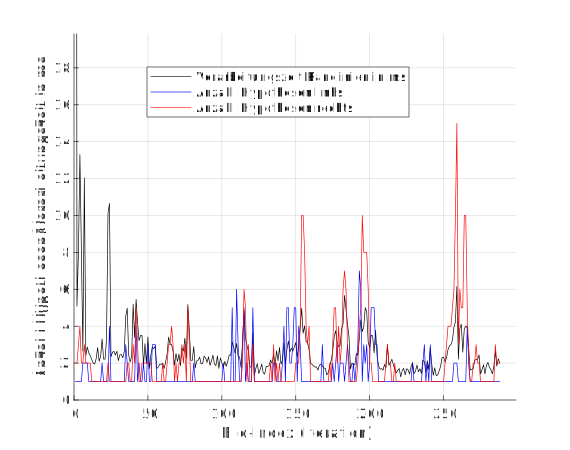
\includegraphics[width=0.5\textwidth]{evaluation_riverflow_hypos_times_04}
\caption{Zusammenhang Anzahl verfolgter Hypothesen \&\ Dauer der Detektion seitlicher Fahrbahnmarkierungen; \SI{4}{cm} Abstand Quader zu Fahrspur}
\label{evaluation:riverflow:hypos:times_04}
\end{figure}

\paragraph{Objekte in der Gegenspur}
Da, bedingt durch die Verifikation, erkannte Fahrbahnmarkierungen nur in die Karte eingetragen werden, wenn sie zu mindestens einer weiteren erkannten Linie passen, muss für eine Fehlerkennung diese Bedingung auch durch die platzierten \glqq Störobjekte\grqq\ erfüllt werden. Da sich das Fahrzeug nur auf der rechten Straßenseite fortbewegt, wurde der Versuchsaufbau in Abb. \ref{fig:evaluation:riverflow:test_kontraste_versuchsaufbau_baustelle} gewählt, welcher diesem Kriterium nachkommt.
\begin{figure}[htbp] % [htb]
\centering
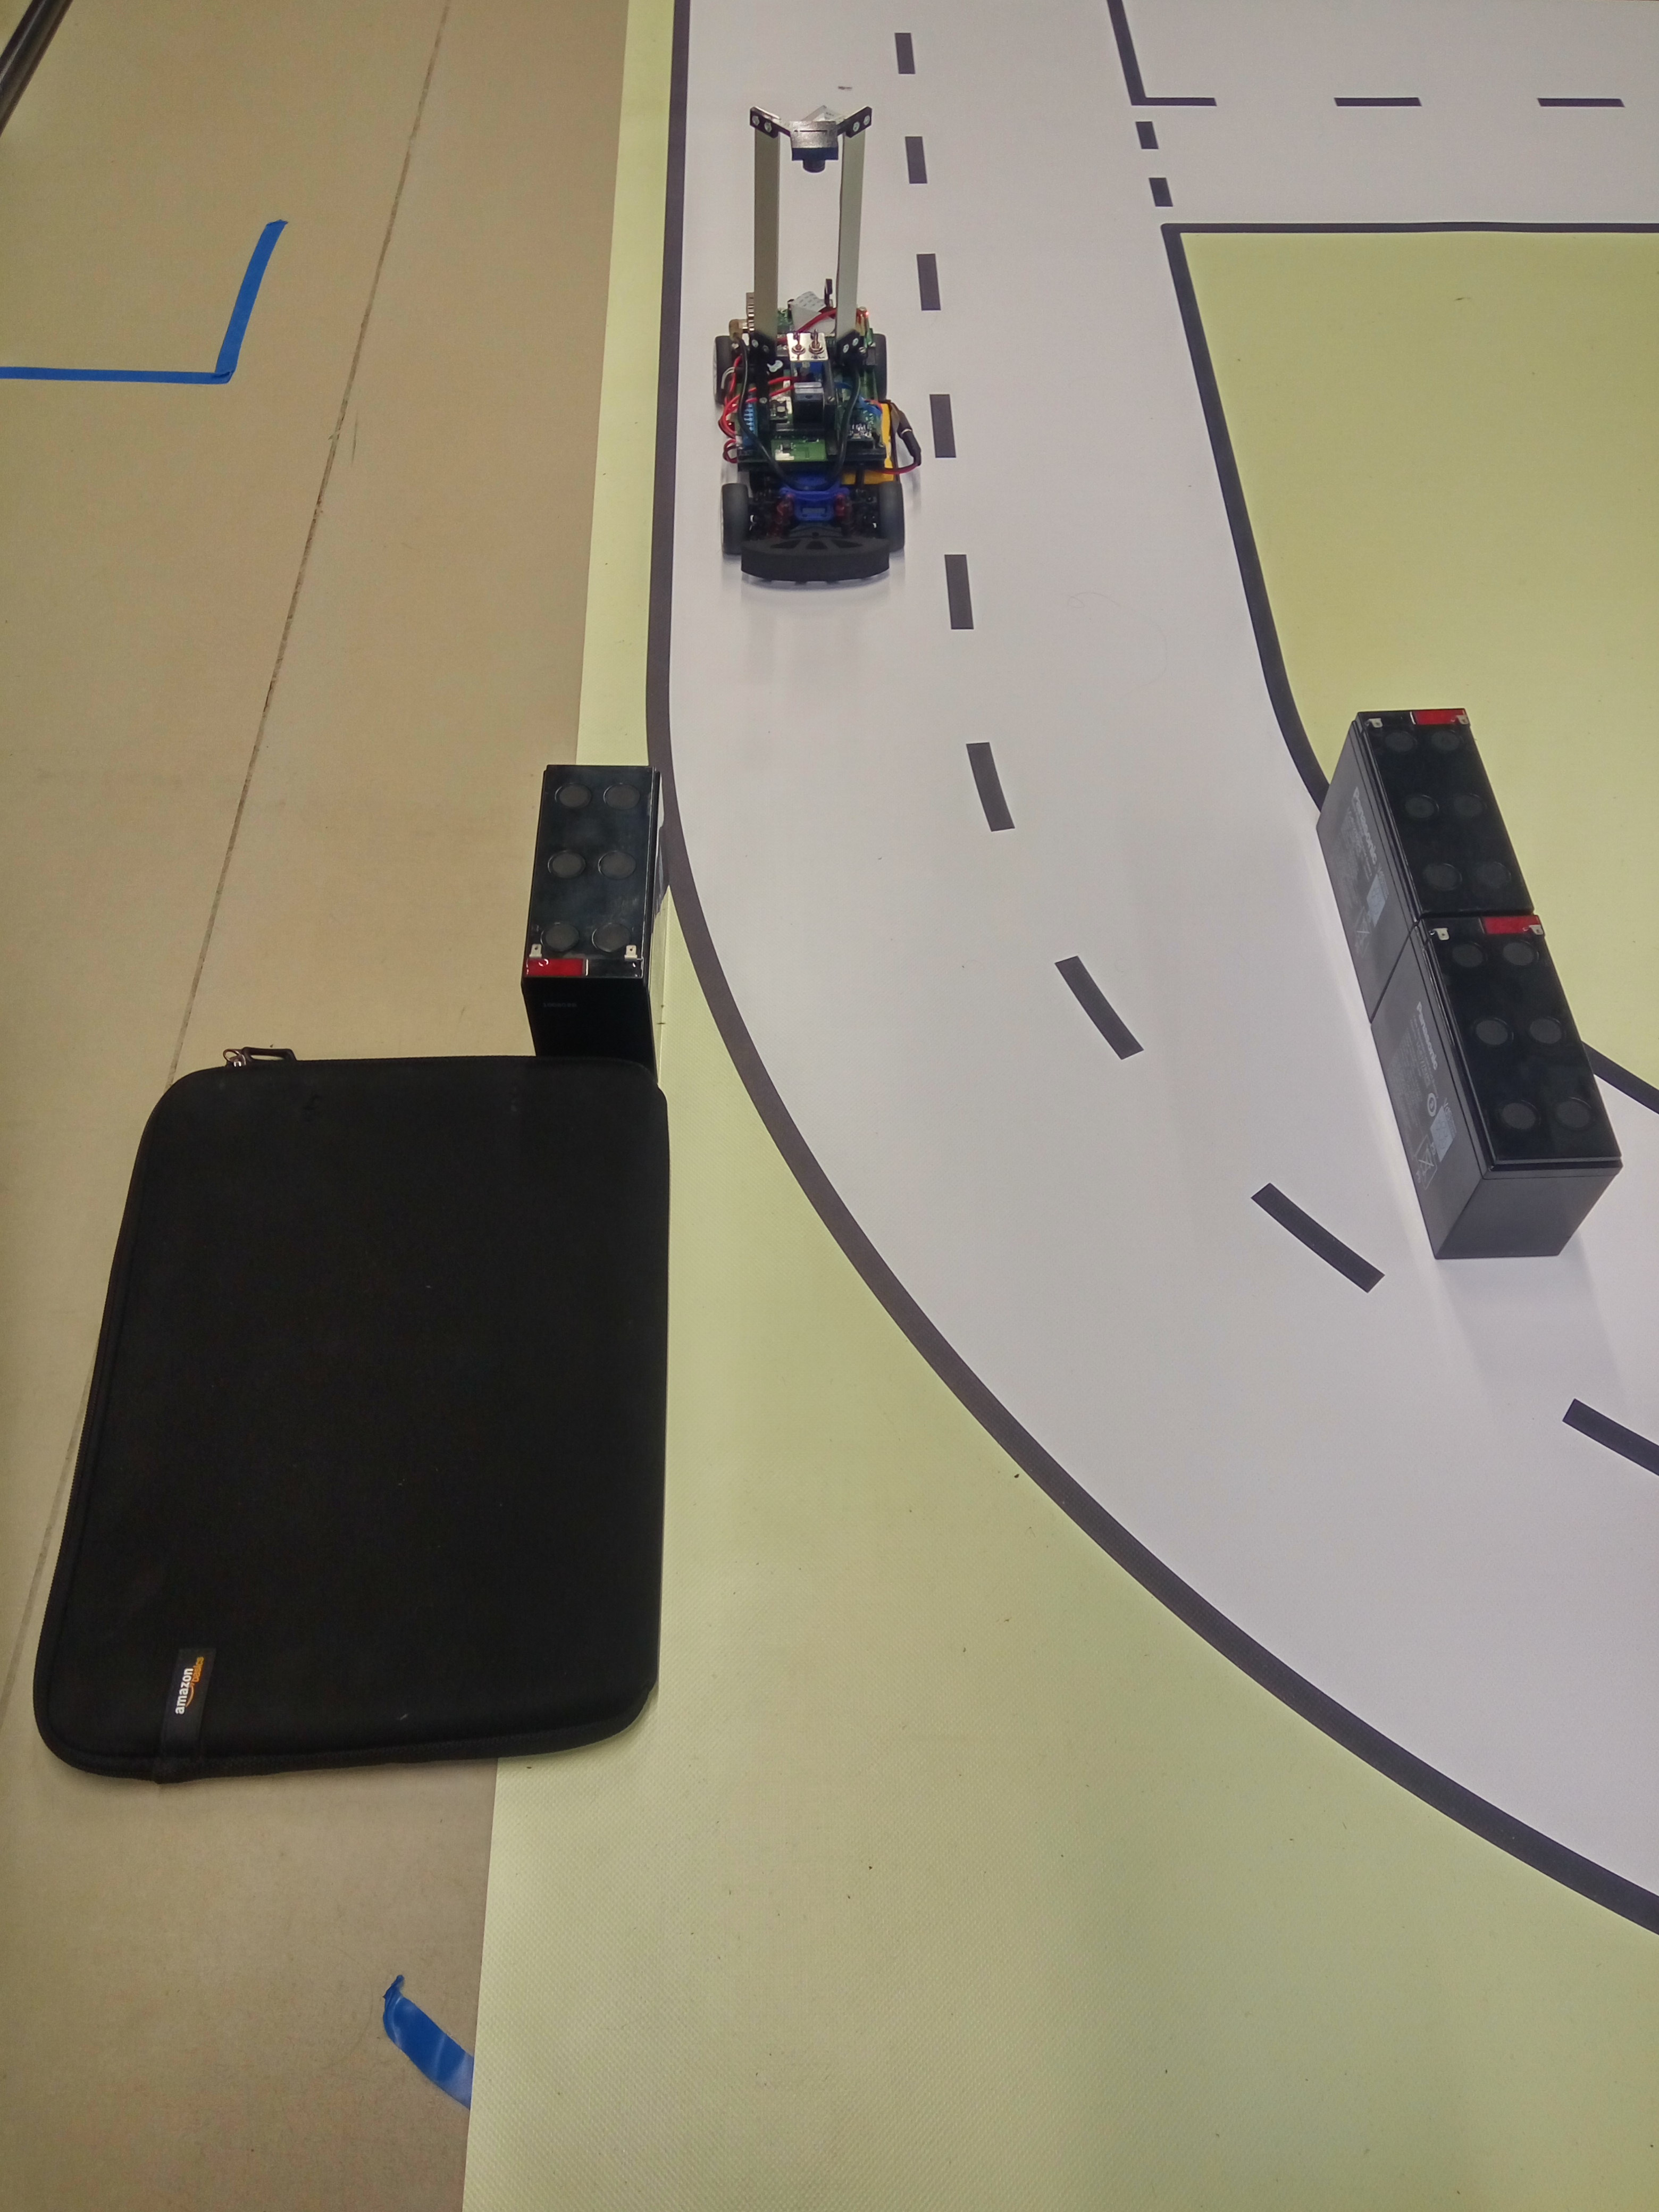
\includegraphics[width=0.5\textwidth]{evaluation_riverflow_test_kontraste_versuchsaufbau_baustelle}
\caption{Versuchsaufbau mit \glqq Störobjekt\grqq\ auf der Gegenfahrspur}
\label{fig:evaluation:riverflow:test_kontraste_versuchsaufbau_baustelle}
\end{figure}

Die Fehldetektion der linken Fahrbahnmarkierung konnte somit provoziert werden. Da die richtig erkannte rechte Randlinie jedoch mehr Punkte generierte und anhand der Mittellinie verifiziert wurde, sind diese zwei Linien noch korrekt in die Weltkarte eingetragen (s. Abb. \ref{fig:evaluation:riverflow:baustelle_weltkarte_1} und \ref{fig:evaluation:riverflow:baustelle_riverflow_plot_1}). Das Modellauto fuhr ein wenig rechts der Ideallinie, kam aber nicht stark vom Kurs ab.
Erst durch Abdecken der Mittellinie (s. Abb. \ref{fig:evaluation:riverflow:baustelle_weltkarte_2} und \ref{fig:evaluation:riverflow:baustelle_riverflow_plot_2}) und die somit fehlende Validierungsmöglichkeit der richtig erkannten rechten Fahrbahnmarkierung konnte der Roboter vom Kurs abgebracht werden und verließ die Straße völlig.
\begin{figure}[htbp] % [htb]
%\centering
%\hfill
\subfloat[Einzelbild mit Mittellinie \label{fig:evaluation:riverflow:baustelle_riverflow_plot_1}]{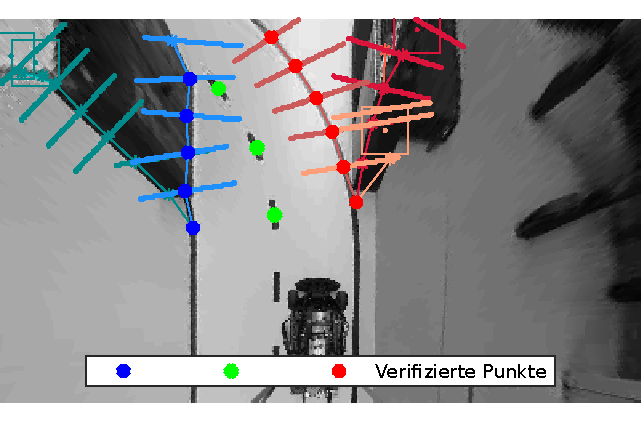
\includegraphics[width=0.49\textwidth]{evaluation_riverflow_baustelle_riverflow_plot_1}}
\hfill
\subfloat[Einzelbild ohne Mittellinie\label{fig:evaluation:riverflow:baustelle_riverflow_plot_2}]{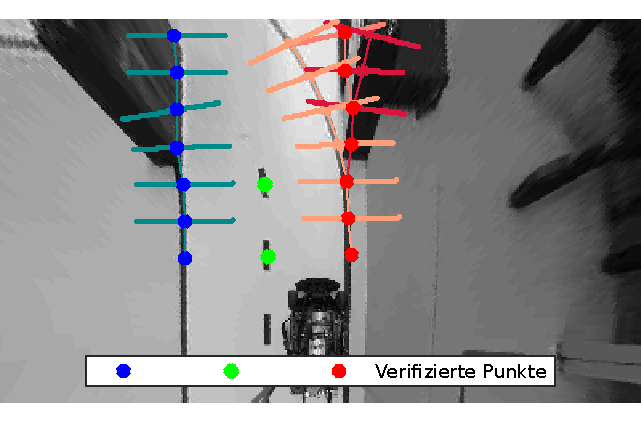
\includegraphics[width=0.49\textwidth]{evaluation_riverflow_baustelle_riverflow_plot_2}}
\hfill
\subfloat[Weltkarte mit Mittellinie\label{fig:evaluation:riverflow:baustelle_weltkarte_1}]{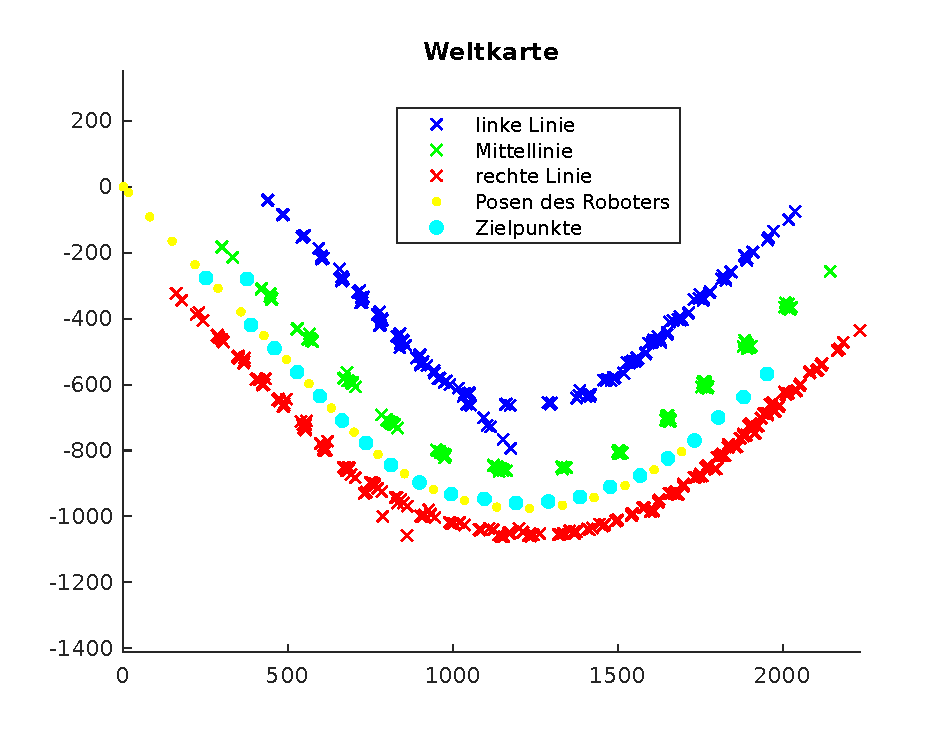
\includegraphics[scale=\mtlstscale]{evaluation_riverflow_baustelle_weltkarte_1}}
\hfill
\subfloat[Weltkarte ohne Mittellinie\label{fig:evaluation:riverflow:baustelle_weltkarte_2}]{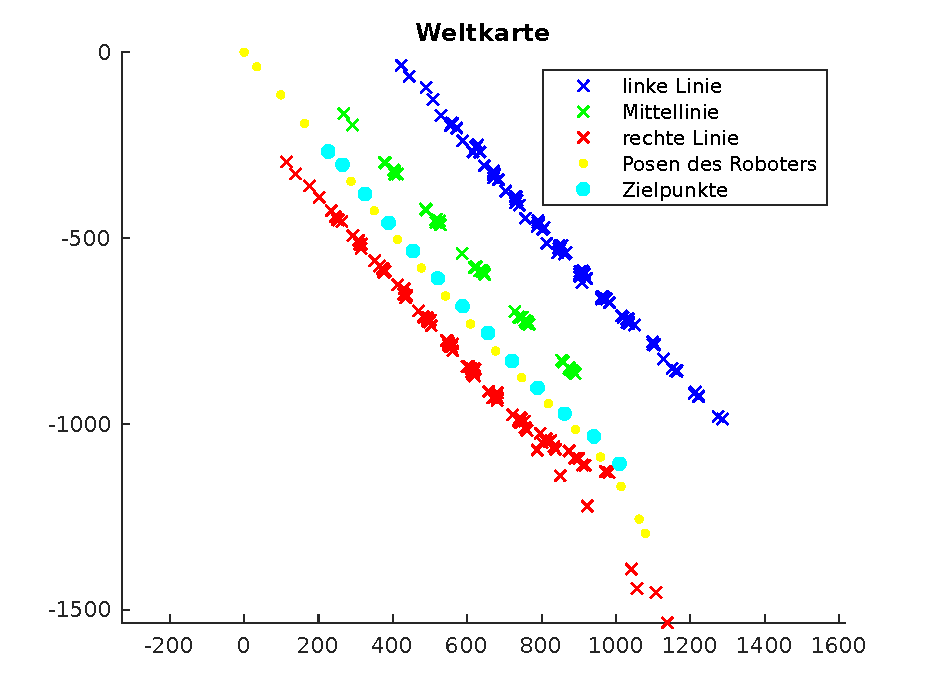
\includegraphics[scale=\mtlstscale]{evaluation_riverflow_baustelle_weltkarte_2}}
%\hfill
\caption{Versuch mit \glqq Störobjekt\grqq\ auf der Gegenfahrspur}
\label{fig:evaluation:riverflow:baustelle}
\end{figure}

\subsection{Fahren mit weniger Informationen \dcfirstauthorshort}
\label{ssec:evaluation:messungen:weniger_infos}
Unsere Linienerkennung besteht im wesentlichen aus den zwei fusionierten Komponenten Mittelstrich- und Randlinienerkennung, was die Robustheit unseres Algorithmus wesentlich erhöht. Um zu zeigen, dass diese nicht nur theoretisch unabhängig voneinander funktionieren, wurden zum Test je einmal die Mittellinie und die beiden Randlinien mit weißem Papier verdeckt. 

%Da unser Algorithmus im wesentlichen aus den zwei nahezu unabhängigen, fusionierten Komponenten für die Mittelstrich- und die Randlinienerkennung besteht, soll in diesem Abschnitt gezeigt werden, dass 

\paragraph{Fahren ohne Mittellinie}
Da in diesem Test keine Mittellinienpunkte gefunden wurden, konnten die Startpunkte für den Riverflow-Algorithmus nur wie in Kapitel~\ref{sssec:fahrspurerkennung:riverflow:randlinie:startpunktgewinnung} beschrieben mittels der vereinfachten Hough-Transformation oder der Annahme fixer Punkte bestimmt werden. Abbildung~\ref{fig:evaluation:riverflow:ohneMittellinie} zeigt den Versuchsaufbau und das Ergebnis der Karte nach einer erfolgreich gefahrenen Runde ohne Mittellinie.

\begin{figure}[htbp] % [htb]
	%\centering
	%\hfill
	\subfloat[Versuchsaufbau ohne Mittellinie \label{fig:evaluation:riverflow:ohneMittellinie:Versuchsaufbau}]{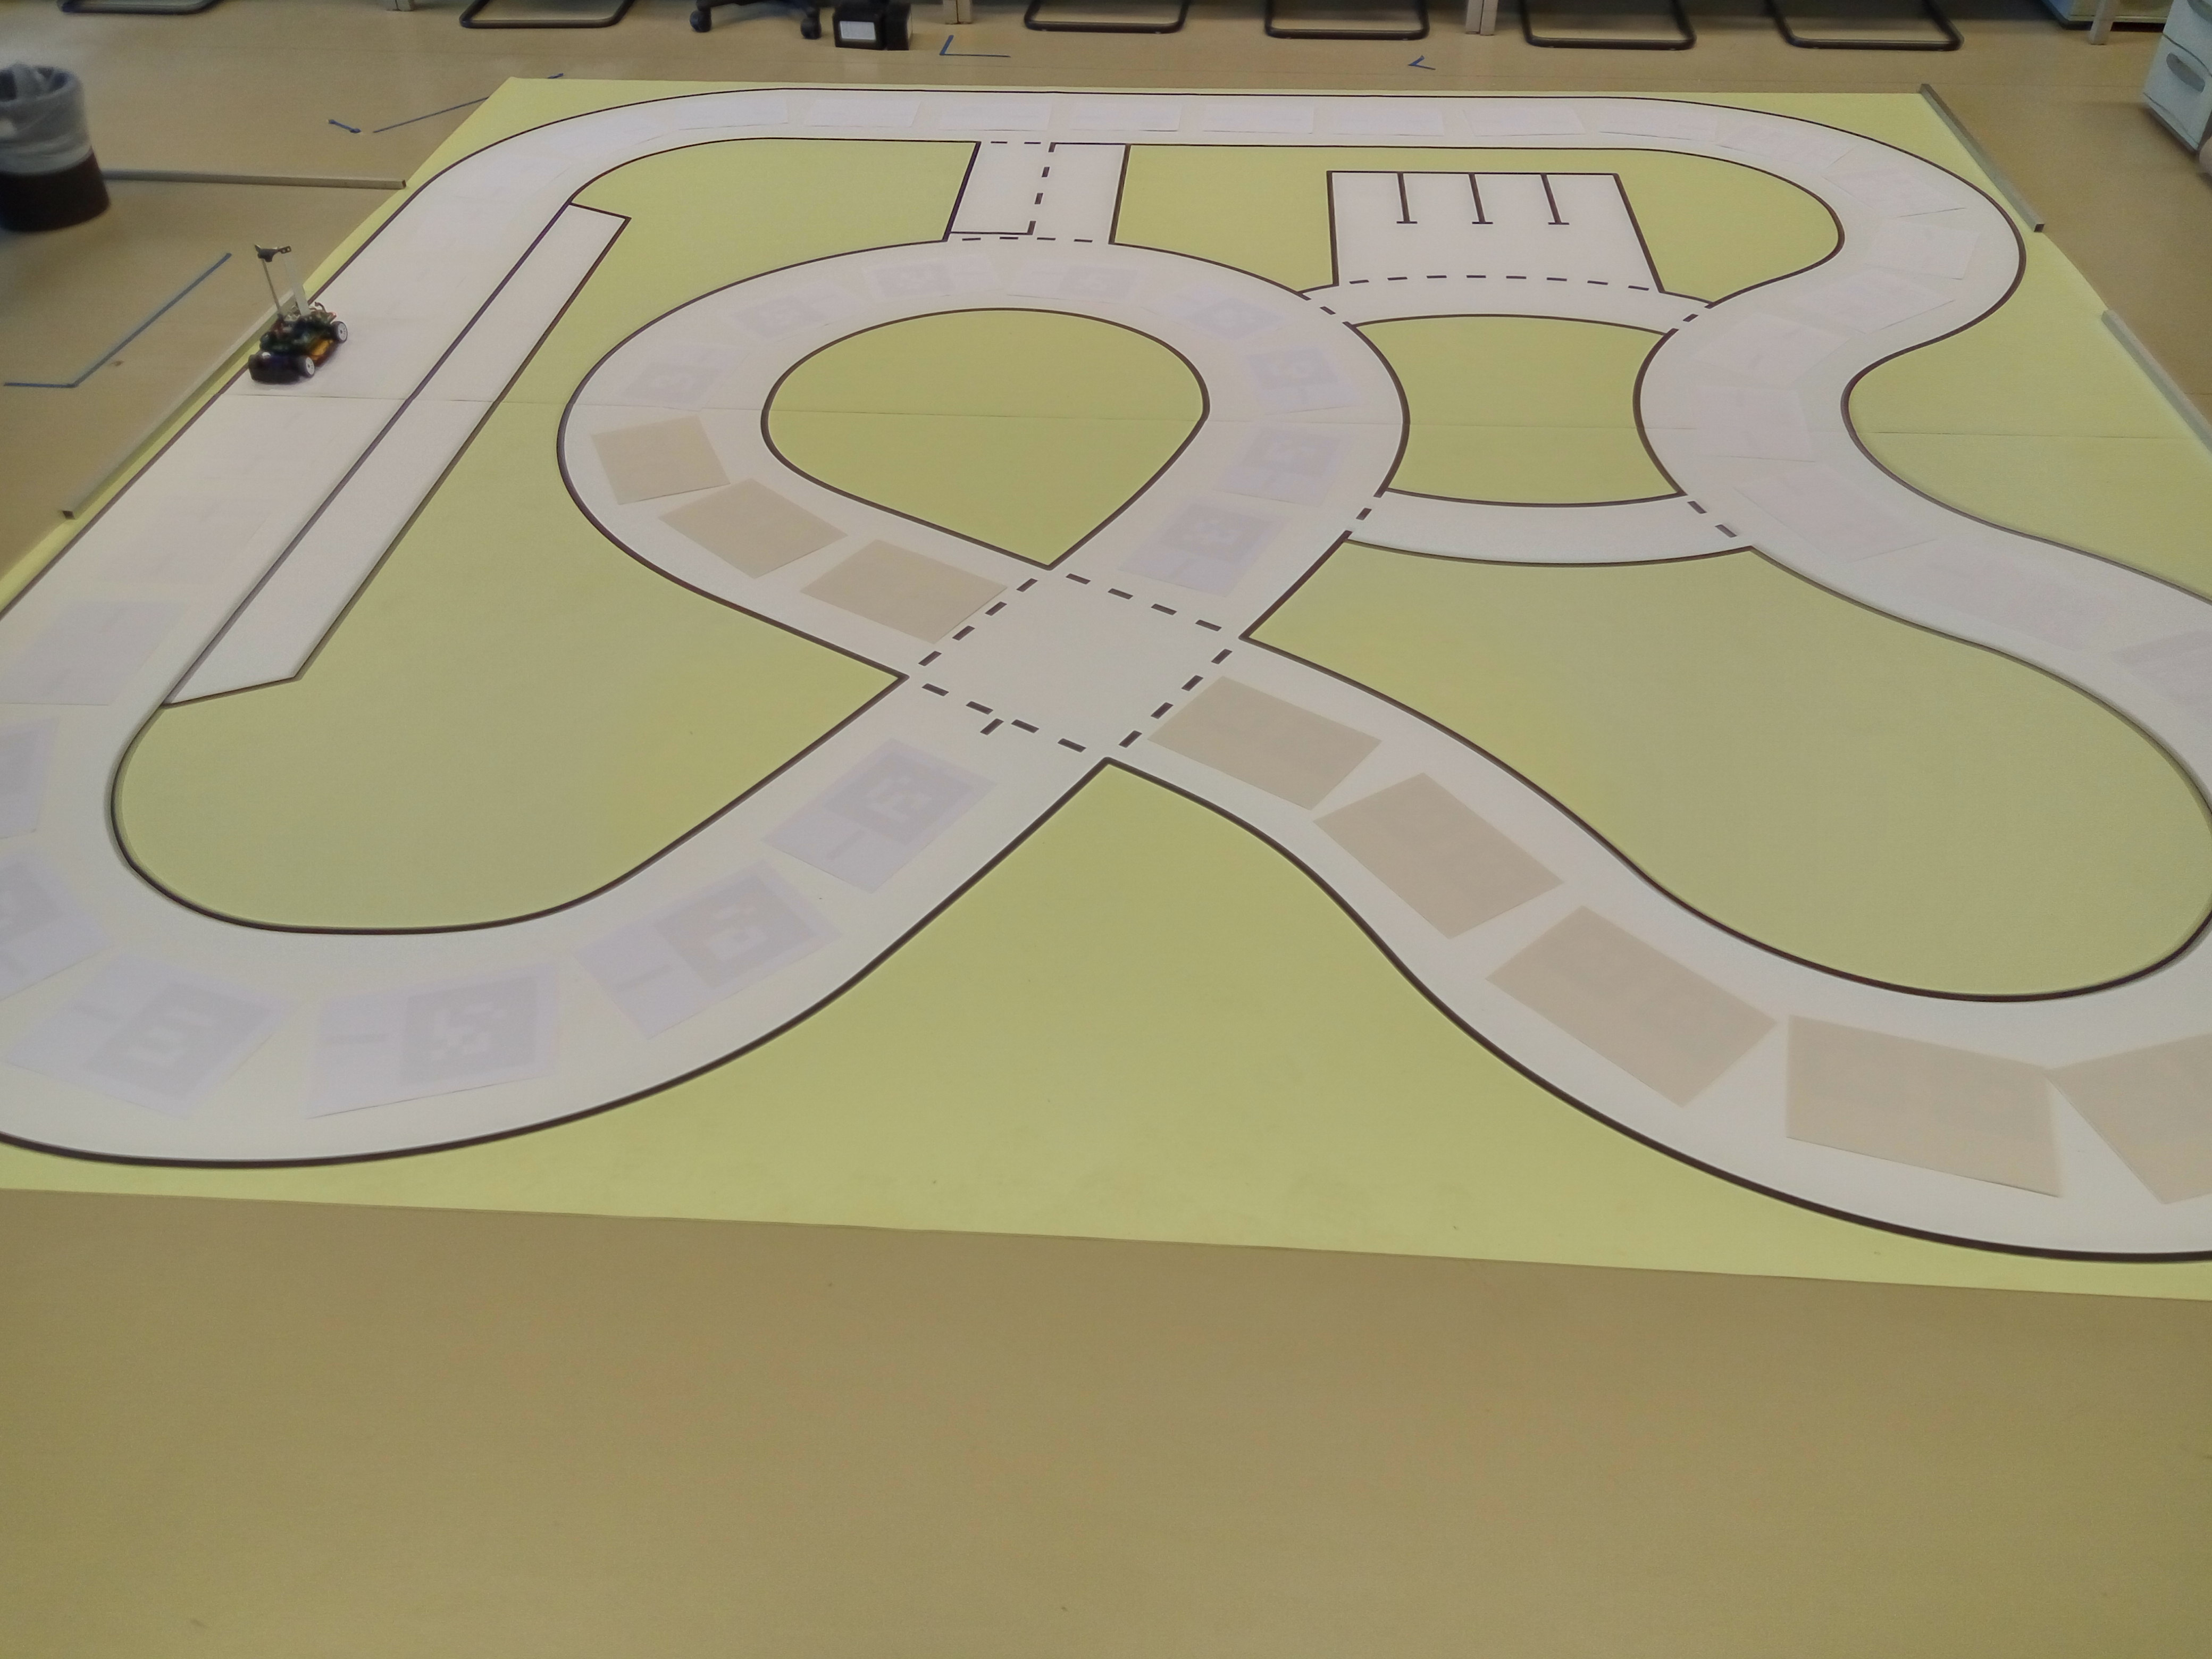
\includegraphics[height=0.28\textheight]{evaluation_riverflow_ohne_mittellinie_versuchsaufbau.jpg}}
	\hfill
	\subfloat[Weltkarte ohne Mittellinie \label{fig:evaluation:riverflow:ohneMittellinie:Weltkarte}]{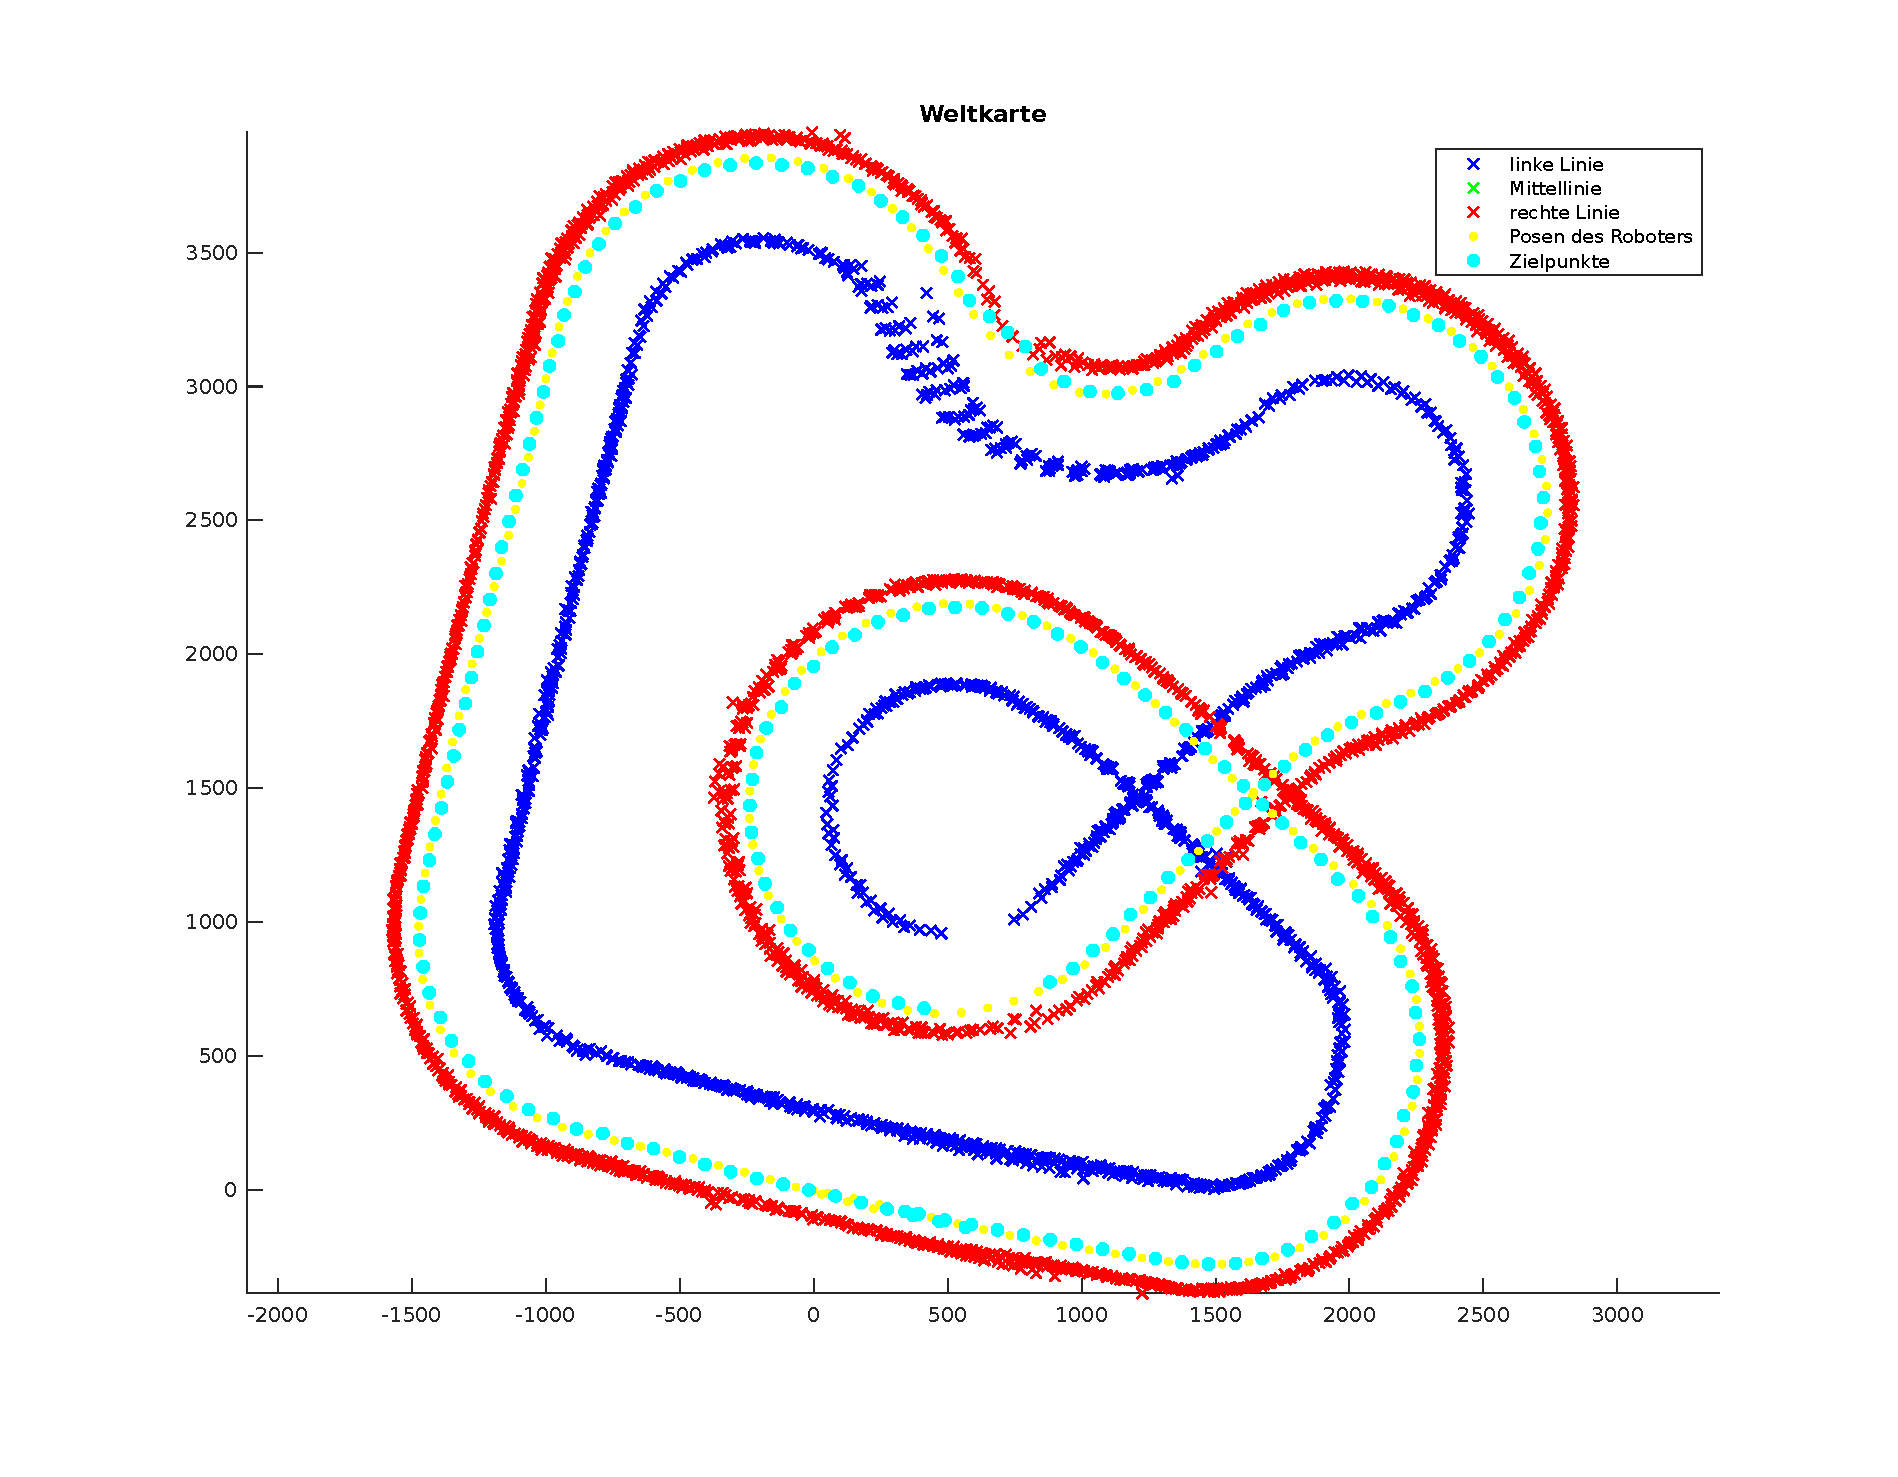
\includegraphics[height=0.28\textheight]{evaluation_riverflow_ohne_mittellinie_worldmap.pdf}}
	\caption{Testfahrt mit durch weißes Papier abgedeckten Mittelstrichen}
	\label{fig:evaluation:riverflow:ohneMittellinie}
\end{figure}

\subparagraph{Probleme}
Damit die gesamte Runde ohne Mittellinie gemeistert werden konnte, wurden während des Versuchs bestimmte Parameter angepasst. Stand der Roboter beispielsweise zu schräg in der Fahrspur, geriet die Randlinie schnell aus dem Bereich, in dem die vereinfachte Hough-Transformation ausgeführt wird. Deshalb wurde die Breite dieses Bildausschnittes vergrößert.%, um sich aus höheren Abweichungen des Fahrzeugs von der Fahrspur wieder fangen zu können. 
Dies führt allerdings zu einem Nachteil, welcher der Grund für die anfangs schmalere Einstellung war und in Abbildung~\ref{fig:evaluation:riverflow:ohneMittellinie:problem} dargestellt ist. Da der Hough-Algorithmus nur nach den größten Maxima sucht (siehe Abschnitt~\ref{ssec:grundlagen:hough:vereinfachte}), erkennt er mitunter bei zu breiter Fenstereinstellung benachbarte Markierungen parallel verlaufender Straßen. Die in Kapitel~\ref{ssec:fahrspurerkennung:riverflow:verifikation} erläuterte Verifikation verhindert erfreulicherweise die Aufnahme der falschen Punkte in die Karte. Da der Roboter jedoch auch keine Richtigen erkannte, erhält er in diesem Fall keine neuen Informationen zur Zielpunktfindung. 

Die Startpunktgewinnung mittels Mittellinie bietet darüber hinaus den großen Vorteil, dass die Richtung des Startpunktvektors bekannt ist. Da diese Information hier fehlt, zeigt der Verschiebungsvektor in x-Richtung des Roboterkoordinatensystems. In engen Kurven führt das in ungünstigen Fällen wie in Abbildung~\ref{fig:evaluation:riverflow:ohneMittellinie:problem} zum Abbruch, da die nächste Scanlinie die Fahrbahnmarkierung nicht mehr schneidet. Das ist der Grund für die große Lücke in der linken Linie der in Abbildung~\ref{fig:evaluation:riverflow:ohneMittellinie:Weltkarte} dargestellten Weltkarte. 

\begin{figure}[htbp] % [htb]
	\centering
	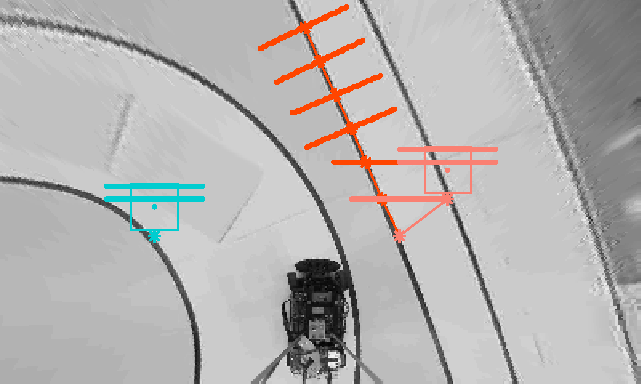
\includegraphics[width=0.7\textwidth]{evaluation_riverflow_ohne_mittellinie_problem_hough.pdf}
	\caption{Ungünstige Position für die mit Hough initialisierte Randlinienerkennung}
	\label{fig:evaluation:riverflow:ohneMittellinie:problem}
\end{figure}

\paragraph{Fahren ohne Randlinien}
Die bisher gute Qualität der binarisierten Bilder ermöglicht eine zuverlässige Mittellinienerkennung. Da diese von keinerlei Startpunkten oder Ähnlichem abhängt, stellen auch enge Kurven oder benachbarte Straßenabschnitte kein Problem dar. Der Versuchsaufbau und die zugehörig aufgenommene Weltkarte sind in Abbildung~\ref{fig:evaluation:riverflow:ohneRandlinie} dargestellt.

\begin{figure}[htbp] % [htb]
%	\centering
	%\hfill
	\subfloat[Versuchsaufbau ohne Randlinien \label{fig:evaluation:riverflow:ohneRandlinie:Versuchsaufbau}]{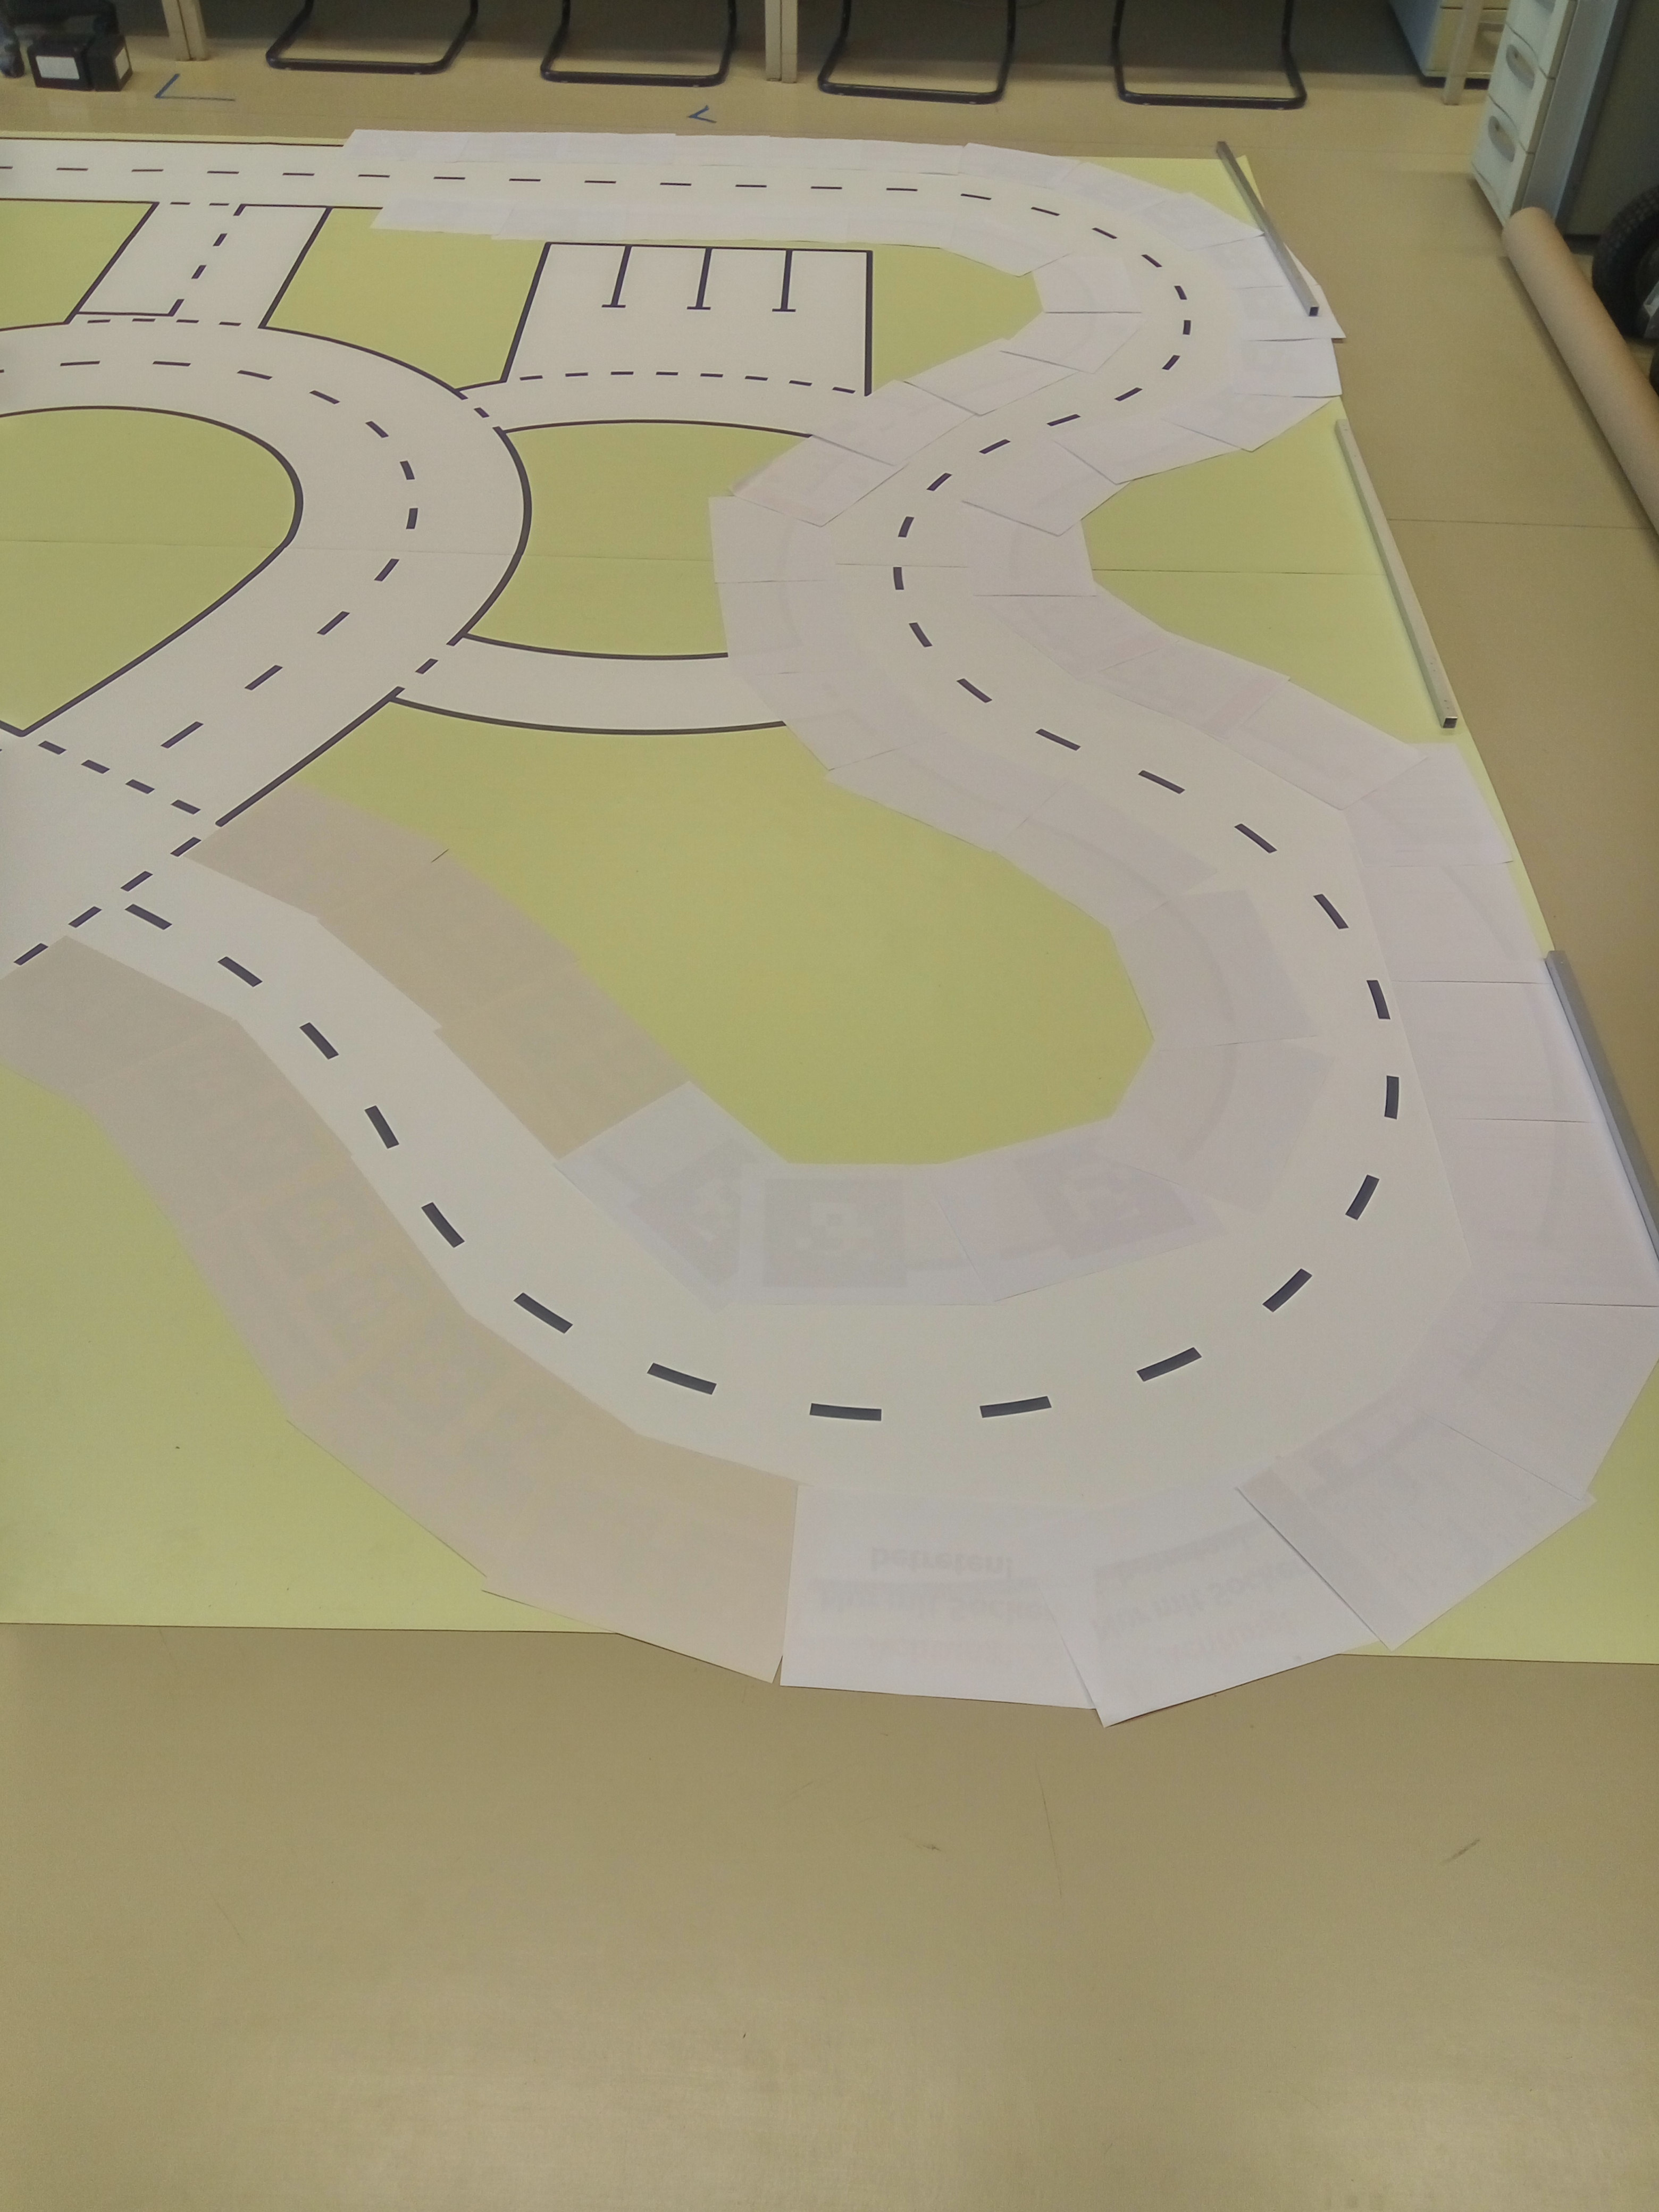
\includegraphics[height=0.35\textheight]{evaluation_riverflow_ohne_randlinie_versuchsaufbau.jpg}}
	\hfill
	\subfloat[Weltkarte ohne Randlinien \label{fig:evaluation:riverflow:ohneRandlinie:Weltkarte}]{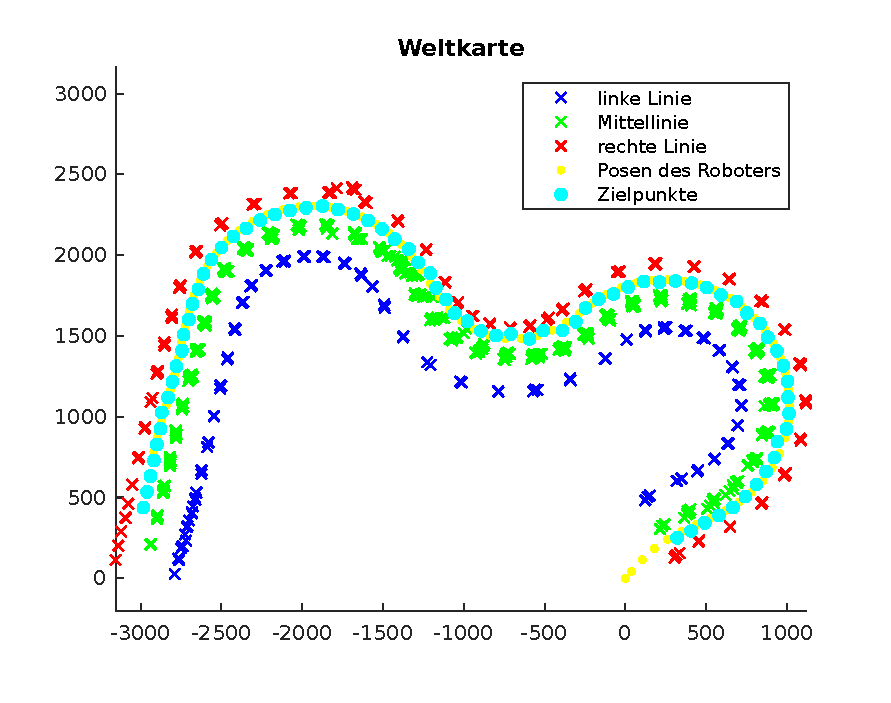
\includegraphics[height=0.35\textheight]{evaluation_riverflow_ohne_randlinie_worldmap.pdf}}
	\caption{Testfahrt mit durch weißes Papier abgedeckte Randlinien}
	\label{fig:evaluation:riverflow:ohneRandlinie}
\end{figure}

Im Plot~\ref{fig:evaluation:riverflow:ohneRandlinie:Weltkarte} fällt auf, dass trotz Abdeckung scheinbar einige Randlinienpunkte erkannt wurden. Mithilfe des in Abbildung~\ref{fig:evaluation:riverflow:ohneMittellinie:bspPlot} dargestellten Beispielplots lässt sich die Erklärung finden.

\begin{figure}[htbp] % [htb]
	\centering
	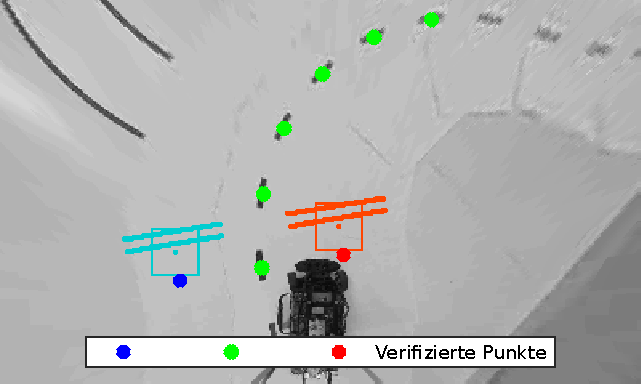
\includegraphics[width=0.7\textwidth]{evaluation_riverflow_ohne_randlinie_beispielplot.pdf}
	\caption{Punkterkennung bei abgedeckten Randlinien}
	\label{fig:evaluation:riverflow:ohneMittellinie:bspPlot}
\end{figure}

Ausgehend von der ersten mittleren Fahrbahnmarkierung werden die Startpunkte für die Randlinienerkennung bestimmt. Trotz fehlender Randlinienpunkte wurden die Startpunkte verifiziert und in die Karte aufgenommen. Da sie jedoch einzig den um die Fahrspurbreite verschobenen Mittellinienpunkt abbilden, stellen sie keinen informativen Mehrwert dar.

\paragraph{Schlussfolgerungen}

Wir haben demonstriert, dass die Rand-und Mittellinienerkennung einzeln funktioniert und sich gegenseitig absichert. Das \gls{glos:tucar} ist nicht auf permanentes Vorhandensein von Mittel-/Randlinien oder deren fehlerfreie Erkennung angewiesen.
Die Zielpunktbestimmung als Voraussetzung für die Regelung ist somit gewährleistet, wenn mindestens die Mittellinie oder beide Randlinien erkannt wurden. Diese Sicherheit ist durch die Schwächen der jeweiligen Verfahren sinnvoll und notwendig. 

An der großen Kreuzung existiert beispielsweise keine mittlere Fahrbahnmarkierung, was die Randlinienerkennung notwendig macht. Gleichzeitig besitzt der Riverflow-Algorithmus den Nachteil, an ausreichend großen Lücken im Markierungsverlauf abzubrechen. Dieser Fall ist demonstrativ in Abbildung~\ref{fig:evaluation:riverflow:Randlinie:unterbrochen:bsp} dargestellt. 

\begin{figure}[htbp] % [htb]
	%\centering
	%\hfill
	\subfloat[Beispielbild einer Unterbrechung \label{fig:evaluation:riverflow:Randlinie:unterbrochen:bsp}]{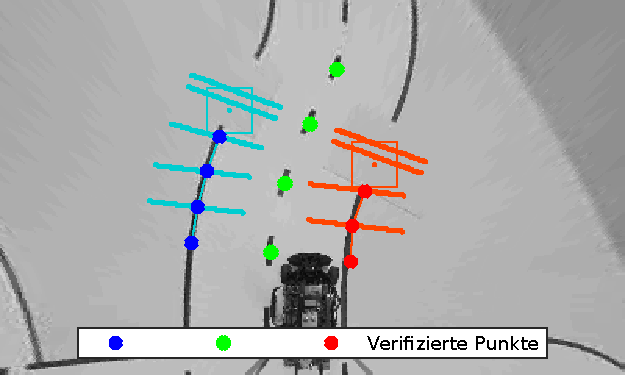
\includegraphics[height=0.25\textheight]{evaluation_riverflow_randlinie_unterbrochen_beispiel.pdf}}
	\hfill
	\subfloat[Länge der erkannten Linien \label{fig:evaluation:riverflow:Randlinie:unterbrochen:linienlaenge}]{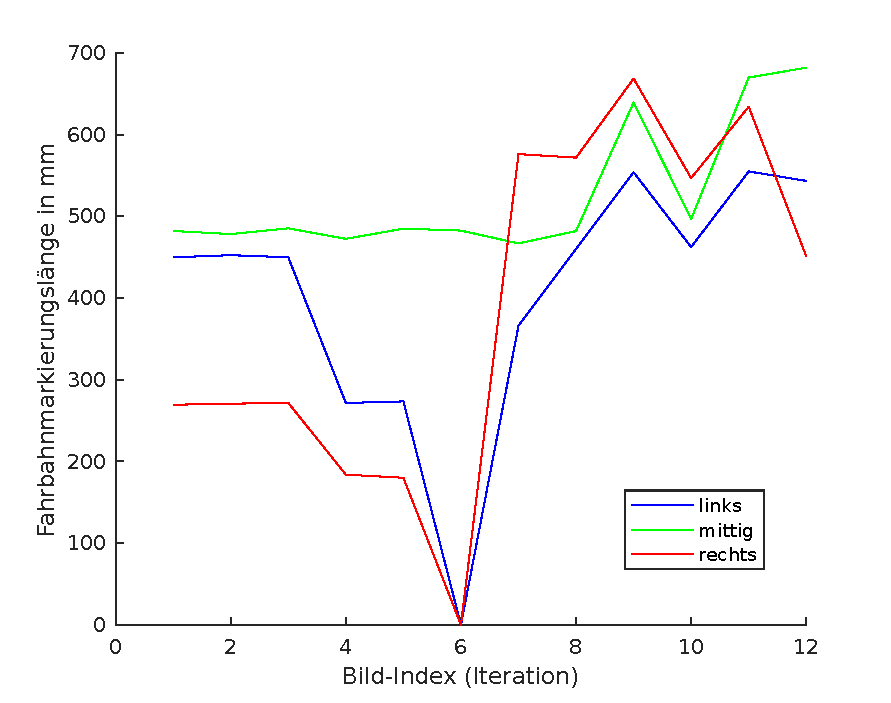
\includegraphics[height=0.25\textheight]{evaluation_riverflow_randlinie_unterbrochen_plot_linienlaenge.pdf}}
	\caption{Demonstration der Schwäche des Riverflow bei größeren Unterbrechungen in der Randlinie}
	\label{fig:evaluation:riverflow:Randlinie:unterbrochen}
\end{figure}

Die durch ein A4-Blatt unterbrochene Randlinie wird im folgenden Verlauf nicht länger erkannt. Dass die Linie in den vorherigen Bilditerationen ebenfalls nur bis zu jener Unterbrechung detektiert wurde, zeigt der Plot in Abbildung \ref{fig:evaluation:riverflow:Randlinie:unterbrochen:linienlaenge} durch die mit jedem Bildindex abnehmende Linienlänge. Die Fähigkeit, mittels Randlinienerkennung vorauszuschauen, ist somit bis zum Passieren dieser Unregelmäßigkeit nicht gegeben. Durch die möglich fehlerhafte Erkennung eines Mittellinienpunktes werden überdies ebenfalls alle nachfolgenden Mittellinienpunkte ignoriert, da auch hier die Verifikation des nächsten Punktes von der des aktuellen abhängt. 

Das unveränderte Szenario lässt die hier beschriebenen Fehler äußerst selten bis gar nicht auftreten. Die jeweils souveräne Rand-und Mittellinienerkennung realisieren die Navigation des \gls{glos:tucar}s sehr robust und zuverlässig. 



%\subsubsection{Leistungsfähigkeit bei Veränderung der Umgebungsbedingungen - Störobjekte}
%Da geplant ist die Teststrecke in Zukunft realistischer zu gestalten, d.h. Objekte wie Straßenschilder, andere Fahrzeuge, Personen und Gebäude hinzuzufügen. Der Einfluss solcher \glqq Störobjekte\grqq\ auf den Fahrspurverfolgungsalgorithmus soll nun untersucht werden.
%
%\paragraph{Menge der Objekte in einem Bild}
%Zu Beginn soll lediglich die Menge der \glqq Störobjekte\grqq\, welche sich in einem Bild befinden, variiert werden. Da sich die Objekte hinreichend weit von der Fahrbahnmarkierung entfernt befinden, ist kein Einfluss die Bildverarbeitung zu erwarten.
%
%\paragraph{Entfernung der Objekte von den Fahrbahnmarkierungen}
%Verringert man die Distanz zwischen \glqq Störobjekten\grqq\ und der Straße, wird es wahrscheinlicher, dass Kanten dieser Gegenstände als Fahrbahnmarkierung erkannt werden.
%
%\paragraph{Kontrast der Objekte im Vergleich zum Testszenario}
%Ist der Helligkeitsunterschied zwischen Fahrbahn und \glqq Störobjekt\grqq\ bzw. der leeren Fläche neben der Fahrbahn und dem \glqq Störobjekt\grqq\ sehr gering, so sollte keine zusätzliche Kante im Bild gefunden und als Fahrbahnmarkierung identifiziert werden . Diese These soll im folgenden Test bestätigt betrachtet werden.
%
%\subsubsection{Leistungsfähigkeit bei Veränderung der Umgebungsbedingungen - fehlende Fahrbahnmarkierungen}
%Es soll gezeigt werden, dass auch bei fehlen bestimmter Fahrbahnmarkierungen eine Verfolgung des Straßenverlaufs möglich ist.






